%%%%%%%%%%%%%%%%%%%%%%%%%%%%%%%%%%%%%%%%%%%%%%%%%%%%%%%%%%%%%%%%%%%%%%%%%%%%%%%%
%
% Template license:
% CC BY-NC-SA 3.0 (http://creativecommons.org/licenses/by-nc-sa/3.0/)
%
%%%%%%%%%%%%%%%%%%%%%%%%%%%%%%%%%%%%%%%%%%%%%%%%%%%%%%%%%%%%%%%%%%%%%%%%%%%%%%%%

%----------------------------------------------------------------------------------------
%	PACKAGES AND OTHER DOCUMENT CONFIGURATIONS
%----------------------------------------------------------------------------------------

\documentclass[
11pt, % The default document font size, options: 10pt, 11pt, 12pt
%oneside, % Two side (alternating margins) for binding by default, uncomment to switch to one side
%chapterinoneline,% Have the chapter title next to the number in one single line
spanish,
singlespacing, % Single line spacing, alternatives: onehalfspacing or doublespacing
%draft, % Uncomment to enable draft mode (no pictures, no links, overfull hboxes indicated)
%nolistspacing, % If the document is onehalfspacing or doublespacing, uncomment this to set spacing in lists to single
%liststotoc, % Uncomment to add the list of figures/tables/etc to the table of contents
%toctotoc, % Uncomment to add the main table of contents to the table of contents
parskip, % Uncomment to add space between paragraphs
%codirector, % Uncomment to add a codirector to the title page
headsepline, % Uncomment to get a line under the header
]{MastersDoctoralThesis} % The class file specifying the document structure



%----------------------------------------------------------------------------------------
%	INFORMACIÓN DE LA MEMORIA
%----------------------------------------------------------------------------------------
\thesistitle{Desarrollo de un \textit{pipeline} de aprendizaje continuo para chatbots basados en PLN} % El títulos de la memoria, se usa en la carátula y se puede usar el cualquier lugar del documento con el comando \ttitle
 

% Nombre del posgrado, se usa en la carátula y se puede usar el cualquier lugar del documento con el comando \degreename
\posgrado{Carrera de Especialización en Inteligencia Artificial} 
%\posgrado{Carrera de Especialización en Internet de las Cosas} 
%\posgrado{Carrera de Especialización en Intelegencia Artificial}
%\posgrado{Maestría en Sistemas Embebidos} 
%\posgrado{Maestría en Internet de las cosas}

\author{Ing. Porra Bustos, Matias Exequiel (UTN-FRLR)} % Tu nombre, se usa en la carátula y se puede usar el cualquier lugar del documento con el comando \authorname

\director{Dr. Ing. Cárdenas Rodrigo (FIUBA)} % El nombre del director, se usa en la carátula y se puede usar el cualquier lugar del documento con el comando \dirname
% \codirector{Nombre del codirector (pertenencia)} % El nombre del codirector si lo hubiera, se usa en la carátula y se puede usar el cualquier lugar del documento con el comando \codirname.  Para activar este campo se debe descomentar la opción "codirector" en el comando \documentclass, línea 23.

\juradoUNO{Nombre del jurado 1 (pertenencia)} % Nombre y pertenencia del un jurado se usa en la carátula y se puede usar el cualquier lugar del documento con el comando \jur1name
\juradoDOS{Nombre del jurado 2 (pertenencia)} % Nombre y pertenencia del un jurado se usa en la carátula y se puede usar el cualquier lugar del documento con el comando \jur2name
\juradoTRES{Nombre del jurado 3 (pertenencia)} % Nombre y pertenencia del un jurado se usa en la carátula y se puede usar el cualquier lugar del documento con el comando \jur3name

\ciudad{Ciudad Autónoma de Buenos Aires}
% \ciudad{ciudad de Mendoza}

\fechaINICIO{mayo de 2024}
\fechaFINAL{abril de 2025}


\keywords{Intelegencia Artificial, FIUBA} % Keywords for your thesis, print it elsewhere with \keywordnames


\begin{document}


\frontmatter % Use roman page numbering style (i, ii, iii, iv...) for the pre-content pages

\pagestyle{plain} % Default to the plain heading style until the thesis style is called for the body content


%----------------------------------------------------------------------------------------
%	RESUMEN - ABSTRACT 
%----------------------------------------------------------------------------------------

\begin{abstract}
\addchaptertocentry{\abstractname} % Add the abstract to the table of contents
%
%The Thesis Abstract is written here (and usually kept to just this page). The page is kept centered vertically so can expand into the blank space above the title too\ldots
\centering

El presente trabajo propone una solución avanzada para la automatización de la comunicación empresarial, orientada a emprendedores y pequeñas empresas. El sistema desarrollado consiste en un chatbot que integra técnicas de procesamiento del lenguaje natural (PLN) y gestión de bases de datos, articulado en un pipeline de aprendizaje continuo. Este chatbot está diseñado para optimizar la interacción con los clientes, generando respuestas precisas y relevantes a sus consultas en lenguaje natural. Además, el sistema se retroalimenta de las interacciones previas para mejorar su rendimiento de manera constante y adaptarse mejor a las necesidades de los usuarios.

\end{abstract}

%----------------------------------------------------------------------------------------
%	CONTENIDO DE LA MEMORIA  - AGRADECIMIENTOS
%----------------------------------------------------------------------------------------

\begin{acknowledgements}
%\addchaptertocentry{\acknowledgementname} % Descomentando esta línea se puede agregar los agradecimientos al índice
\vspace{1.5cm}

% Esta sección es para agradecimientos personales y es totalmente \textbf{OPCIONAL}.  
A mi novia por apoyo incondicional durante todo el proceso de desarrollo de este trabajo. 

A mi familia, por estar siempre presente. 

A mi tutor, por su guía y su conocimiento.

A Michael Schreiber por sus grandes aportes y guía en mi formación profesional en IA. 

\end{acknowledgements}

%----------------------------------------------------------------------------------------
%	LISTA DE CONTENIDOS/FIGURAS/TABLAS
%----------------------------------------------------------------------------------------

\tableofcontents % Prints the main table of contents

\listoffigures % Prints the list of figures

\listoftables % Prints the list of tables


%----------------------------------------------------------------------------------------
%	CONTENIDO DE LA MEMORIA  - DEDICATORIA
%----------------------------------------------------------------------------------------

% \dedicatory{\textbf{Dedicado a... [OPCIONAL]}}  % escribir acá si se desea una dedicatoria

%----------------------------------------------------------------------------------------
%	CONTENIDO DE LA MEMORIA  - CAPÍTULOS
%----------------------------------------------------------------------------------------

\mainmatter % Begin numeric (1,2,3...) page numbering

\pagestyle{thesis} % Return the page headers back to the "thesis" style

% Incluir los capítulos como archivos separados desde la carpeta Chapters

% Chapter 1

\chapter{Introducción general} % Main chapter title

\label{Chapter1} % For referencing the chapter elsewhere, use \ref{Chapter1} 
\label{IntroGeneral}


%----------------------------------------------------------------------------------------

% Define some commands to keep the formatting separated from the content 
\newcommand{\keyword}[1]{\textbf{#1}}
\newcommand{\tabhead}[1]{\textbf{#1}}
\newcommand{\code}[1]{\texttt{#1}}
\newcommand{\file}[1]{\texttt{\bfseries#1}}
\newcommand{\option}[1]{\texttt{\itshape#1}}
\newcommand{\grados}{$^{\circ}$}

%----------------------------------------------------------------------------------------

%\section{Introducción}

%----------------------------------------------------------------------------------------
% \section{Resumen inicial{}}
En este capítulo se exploran las motivaciones que impulsaron el desarrollo del sistema, diseñado para automatizar la comunicación entre emprendedores y sus clientes. Se ofrece, además, una explicación detallada sobre qué son los chatbots y las razones por las que su uso resulta fundamental en este contexto. Finalmente, se describen los objetivos principales del trabajo, centrados en la facilidad de implementación y en la mejora de la eficiencia operativa, junto con el alcance definido durante la planificación.

\section{Motivación{}}

El sistema desarrollado en el presente trabajo surge de la necesidad de proporcionar a emprendedores una herramienta que les permita automatizar la comunicación con sus clientes de manera eficiente y personalizada. Esta herramienta les ofrece una ventaja competitiva al optimizar la gestión de sus interacciones con los usuarios y les permite mejorar la eficiencia operativa, además de reducir los costos asociados a la atención al cliente.


\subsection{¿Qué es un chatbot?}

Un chatbot es un programa de software que emplea técnicas de Procesamiento del Lenguaje Natural (PLN)\footnote{El procesamiento de lenguaje natural, o PLN, combina la lingüística computacional (modelado del lenguaje humano basado en reglas) con modelos estadísticos y de aprendizaje automático para permitir que las computadoras y los dispositivos digitales reconozcan, comprendan y generen texto y voz. \url{https://www.ibm.com/mx-es/topics/natural-language-processing}} para interpretar y contestar automáticamente las consultas de los usuarios de manera coherente y eficiente. Esto facilita la automatización de interacciones comunes y mejora la experiencia del cliente.

\subsubsection{¿Por qué un chatbot?}

A continuación, se destacan algunas de las razones principales por las cuales un chatbot es la solución ideal para este trabajo:

\begin{itemize}
    \item Disponibilidad 24/7: los chatbots están disponibles en todo momento, lo que permite a las empresas atender consultas de sus clientes a cualquier hora del día.
    
    \item Reducción de costos: al automatizar la atención al cliente, los chatbots permiten a las empresas reducir los costos asociados a personal humano, sin comprometer la calidad del servicio.
    
    \item Recolección de datos valiosos: los chatbots pueden recopilar y analizar información relevante sobre las interacciones con los clientes, lo que permite a las empresas ajustar sus estrategias de manera eficiente.
    
    \item Optimización de tiempos de respuesta: la capacidad de generar respuestas inmediatas en función de consultas predefinidas optimiza los tiempos de respuesta.
\end{itemize}

% \subsection{Guía matemática rápida para \LaTeX{}}

% Si estás escribiendo un documento con mucho contenido matemático, entonces es posible que desees leer el documento de la AMS (American Mathematical Society) llamado, \enquote{A Short Math Guide for \LaTeX{}}. Se puede encontrar en línea en el siguiente link: \url{http://www.ams.org/tex/amslatex.html} en la sección \enquote{Additional Documentation} hacia la parte inferior de la página.


%----------------------------------------------------------------------------------------
% \newpage % agrego un salto de página 
\subsection{Objetivos principales}

El trabajo se enfoca en tres objetivos principales que se interrelacionan para ofrecer una solución integral a pequeños emprendedores. Cada uno de estos objetivos está orientado a asegurar que la herramienta sea accesible, fácilmente implementable y de bajo costo, para garantizar una experiencia eficiente y optimizada para las empresas que la adopten. 
 
A continuación, se detallan los objetivos principales:


\begin{itemize}
    \item Hacer accesible la solución a pequeños emprendedores: desarrollar un sistema que sea de fácil adopción y pueda ser utilizado por pequeñas empresas, independientemente de sus conocimientos técnicos.
    
    \item Garantizar una fácil implementación: diseñar una solución replicable, de manera que cualquier empresa pueda contar con el chatbot simplemente proporcionando el contexto necesario para su entrenamiento. No será necesario disponer de infraestructura compleja ni personal especializado.
    
    \item Reducir el costo de mantenimiento: proporcionar una herramienta con un bajo costo de mantenimiento, tanto en términos económicos como de tiempo, para que los emprendedores puedan centrarse en su negocio principal.
    
\end{itemize}


% Incluir aquí el gráfico de Venn que detalle la relación de los objetivos principales.
% \includegraphics[width=\textwidth]{ruta/al/grafico_venn.png}

\begin{figure}[htbp]

  \centering
  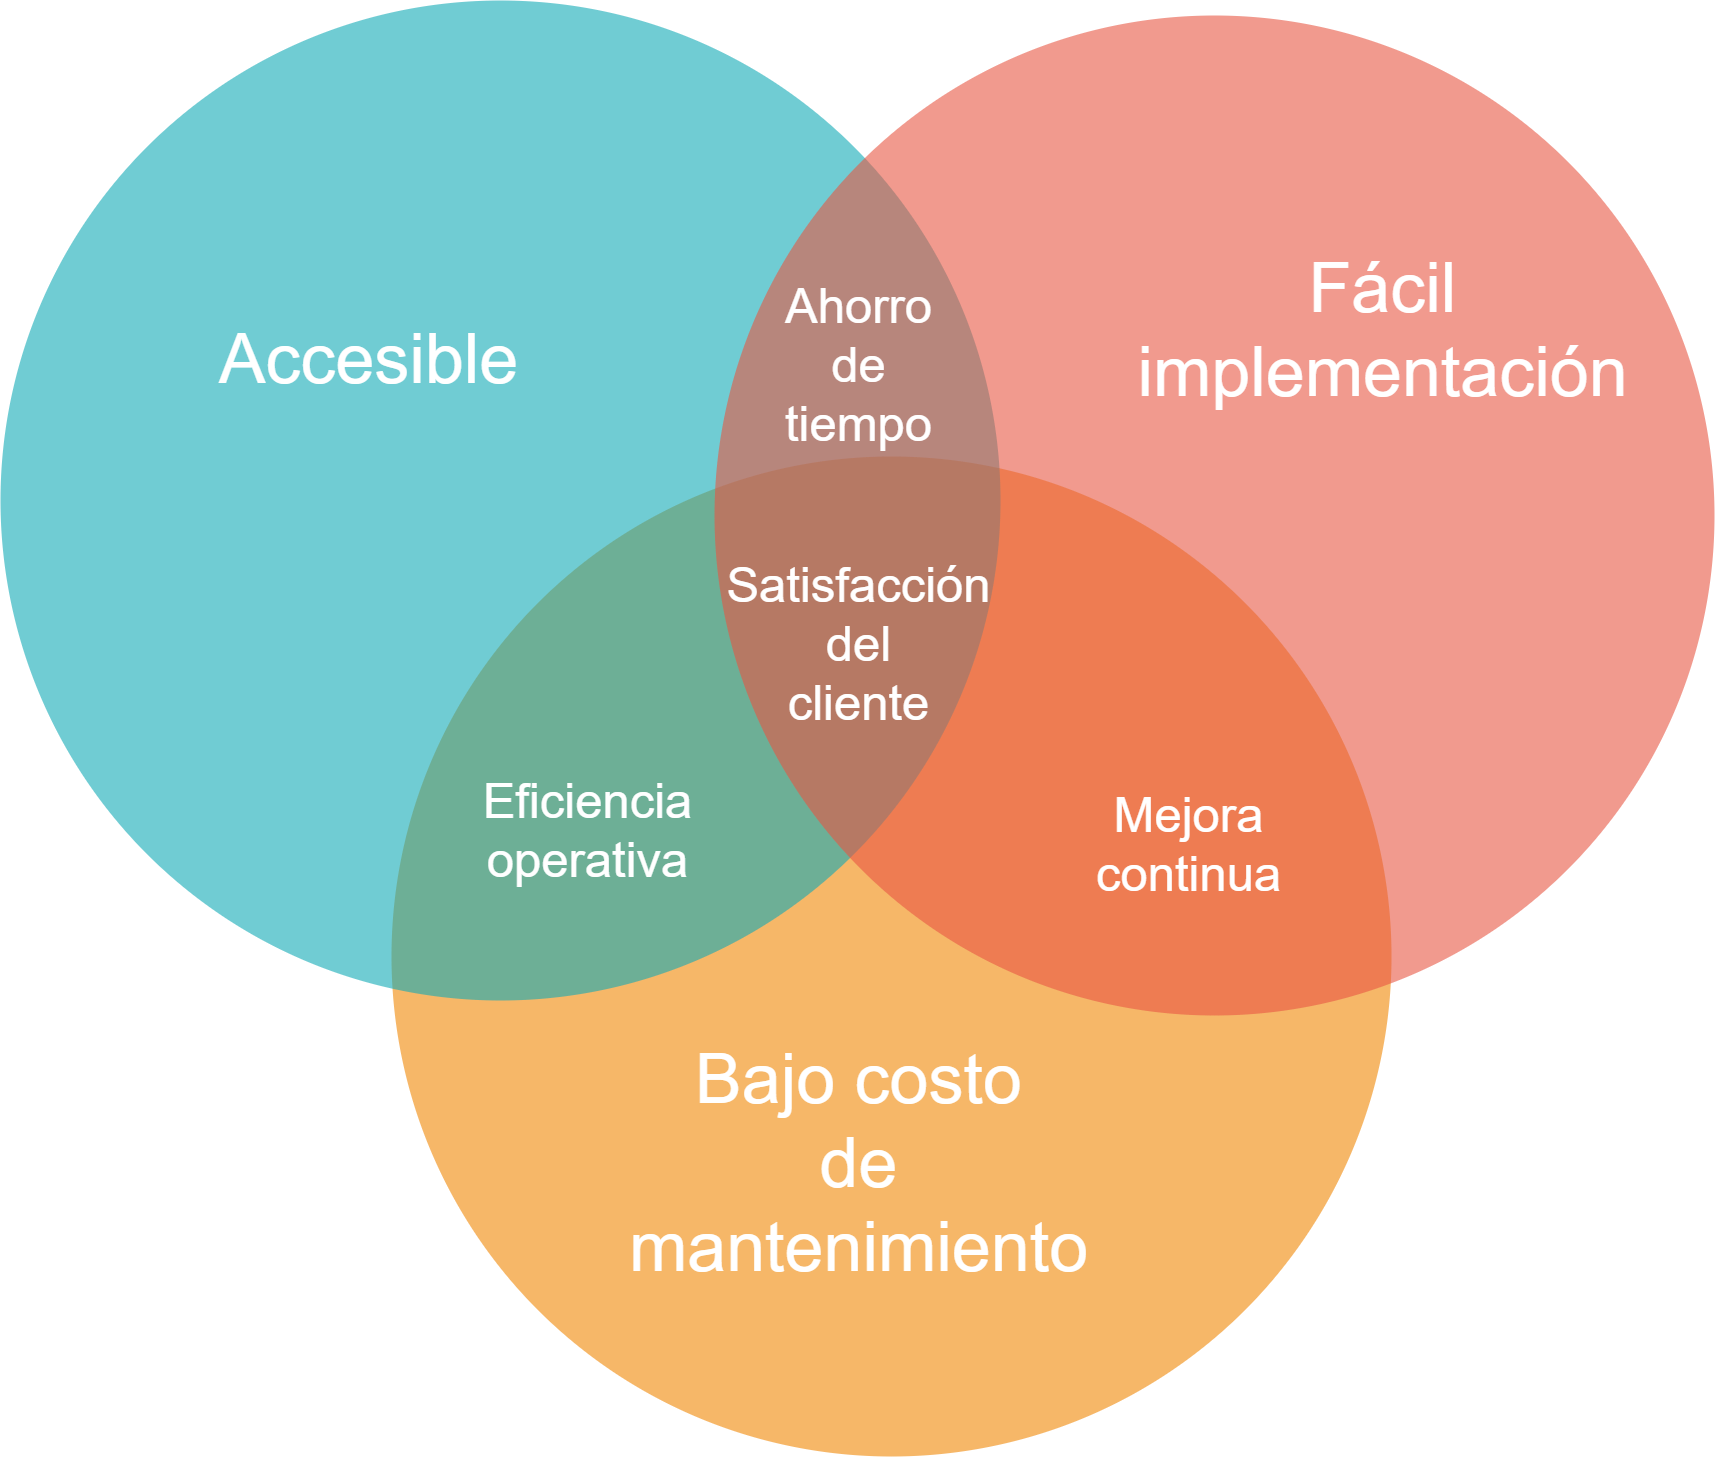
\includegraphics[width=.75\textwidth]{./Figures/Venn_objetivos.png}
  \caption{Relación entre los objetivos centrales.}
  \label{fig:objetivos_venn}
\end{figure}

\subsection{Alcance del trabajo}

Durante la planificación del trabajo se propusieron las siguientes actividades:

\begin{itemize}
    \item Diseño, desarrollo e implementación de un \textit{pipeline} completo para la creación y gestión de chatbots basados en PLN, con capacidad de aprendizaje continuo.
    \item Desarrollo de algoritmos para el preprocesamiento de información y generación de respuestas relevantes y coherentes.
    \item Establecimiento de métricas y procedimientos de evaluación para medir la calidad y eficacia de las respuestas del chatbot.
    \item Implementación de un sistema de retroalimentación que utilice los datos de interacciones con usuarios para mejorar el rendimiento del modelo.
\end{itemize}

Se espera que los resultados incluyan un sistema accesible, de fácil implementación y de bajo costo, que permita a los emprendedores mejorar la eficiencia de sus comunicaciones con los clientes, ahorrando tiempo y mejorando la satisfacción del cliente.



% Si estás familiarizado con \LaTeX{}, entonces podés explorar la estructura de directorios de esta plantilla y proceder a personalizarla agregando tu información en el bloque \emph{INFORMACIÓN DE LA PORTADA} en el archivo \file{memoria.tex}.  

% Se puede continuar luego modificando el resto de los archivos siguiendo los lineamientos que se describen en la sección \ref{sec:FillingFile} en la página \pageref{sec:FillingFile}.

% Debés asegurarte de leer el capítulo \ref{Chapter2} acerca de las convenciones utilizadas para las Memoria de los Trabajos Finales de la \degreename.

% Si sos nuevo en \LaTeX{}, se recomienda que continúes leyendo el documento ya que contiene información básica para aprovechar el potencial de esta herramienta.


%----------------------------------------------------------------------------------------

\section{Estado del arte}
 
\subsection{Revisión de tecnologías}
...
% Esta plantilla se distribuye como una único archivo .zip que se puede descomprimir en varios archivos y carpetas. Asimismo, se puede consultar el repositorio git para obtener la última versión de los archivos, \url{https://github.com/patriciobos/Plantilla-CESE.git}. Los nombres de las carpetas son, o pretender ser, auto-explicativos.

% \keyword{Appendices} -- Esta es la carpeta donde se deben poner los apéndices. Cada apéndice debe ir en su propio archivo \file{.tex}. Se incluye un ejemplo y una plantilla en la carpeta.

% \keyword{Chapters} -- Esta es la carpeta donde se deben poner los capítulos de la memoria. Cada capítulo debe ir un su propio archivo \file{.tex} por separado.  Se ofrece por defecto, la siguiente estructura de capítulos y se recomienda su utilización dentro de lo posible:

% \begin{itemize}
% \item Capítulo 1: Introducción general	
% \item Capítulo 2: Introducción específica
% \item Capítulo 3: Diseño e implementación
% \item Capítulo 4: Ensayos y resultados
% \item Capítulo 5: Conclusiones

% \end{itemize}

% Esta estructura de capítulos es la que se recomienda para las memorias de la especialización.

% \keyword{Figures} -- Esta carpeta contiene todas las figuras de la memoria.  Estas son las versiones finales de las imágenes que van a ser incluidas en la memoria.  Pueden ser imágenes en formato \textit{raster}\footnote{\url{https://en.wikipedia.org/wiki/Raster_graphics}} como \file{.png}, \file{.jpg} o en formato vectoriales\footnote{\url{https://en.wikipedia.org/wiki/Vector_graphics}} como \file{.pdf}, \file{.ps}.  Se debe notar que utilizar imágenes vectoriales disminuye notablemente el peso del documento final y acelera el tiempo de compilación por lo que es recomendable su utilización siempre que sea posible.

\subsection{investigaciones previas y tendencias actuales}

...
% También están incluidos varios archivos, la mayoría de ellos son de texto plano y se puede ver su contenido en un editor de texto. Después de la compilación inicial, se verá que más archivos auxiliares son creados por \ LaTeX{} o BibTeX, pero son de uso interno y no es necesario hacer nada en particular con ellos.  Toda la información necesaria para compilar el documento se encuentra en los archivos \file{.tex}, \file{.bib}, \file{.cls} y en las imágenes de la carpeta Figures.

% \keyword{referencias.bib} - este es un archivo importante que contiene toda la información de referencias bibliográficas que se utilizarán para las citas en la memoria en conjunto con BibTeX. Usted puede escribir las entradas bibliográficas en forma manual, aunque existen también programas de gestión de referencias que facilitan la creación y gestión de las referencias y permiten exportarlas en formato BibTeX.  También hay disponibles sitios web como \url{books.google.com} que permiten obtener toda la información necesaria para una cita en formato BibTeX. Ver sección \ref{sec:biblio}

% \keyword{MastersDoctoralThesis.cls} -- este es un archivo importante. Es el archivos con la clase que le informa a \LaTeX{} cómo debe dar formato a la memoria. El usuario de la plantilla no debería necesitar modificar nada de este archivo.

% \keyword{memoria.pdf} -- esta es su memoria con una tipografía bellamente compuesta (en formato de archivo PDF) creado por \LaTeX{}. Se distribuye con la plantilla y después de compilar por primera vez sin hacer ningún cambio se debería obtener una versión idéntica a este documento.

% \keyword{memoria.tex} -- este es un archivo importante. Este es el archivo que tiene que compilar \LaTeX{} para producir la memoria como un archivo PDF. Contiene un marco de trabajo y estructuras que le indican a \LaTeX{} cómo diagramar la memoria.  Está altamente comentado para que se pueda entender qué es lo que realiza cada línea de código y por qué está incluida en ese lugar.  En este archivo se debe completar la información personalizada de las primeras sección según se indica en la sección \ref{sec:FillingFile}.

% Archivos que \emph{no} forman parte de la distribución de la plantilla pero que son generados por \LaTeX{} como archivos auxiliares necesarios para la producción de la memoria.pdf son:

% \keyword{memoria.aux} -- este es un archivo auxiliar generado por \LaTeX{}, si se borra \LaTeX{} simplemente lo regenera cuando se compila el archivo principal \file{memoria.tex}.

% \keyword{memoria.bbl} -- este es un archivo auxiliar generado por BibTeX, si se borra BibTeX simplemente lo regenera cuando se compila el archivo principal \file{memoria.tex}. Mientras que el archivo \file{.bib} contiene todas las referencias que hay, este archivo \file{.bbl} contine sólo las referencias que han sido citadas y se utiliza para la construcción de la bibiografía.

% \keyword{memoria.blg} -- este es un archivo auxiliar generado por BibTeX, si se borra BibTeX simplemente lo regenera cuando se compila el archivo principal \file{memoria.tex}.

% \keyword{memoria.lof} -- este es un archivo auxiliar generado por \LaTeX{}, si se borra \LaTeX{} simplemente lo regenera cuando se compila el archivo principal \file{memoria.tex}.  Le indica a \LaTeX{} cómo construir la sección \emph{Lista de Figuras}.
 
% \keyword{memoria.log} --  este es un archivo auxiliar generado por \LaTeX{}, si se borra \LaTeX{} simplemente lo regenera cuando se compila el archivo principal \file{memoria.tex}. Contiene mensajes de \LaTeX{}. Si se reciben errores o advertencias durante la compilación, se guardan en este archivo \file{.log}.

% \keyword{memoria.lot} -- este es un archivo auxiliar generado por \LaTeX{}, si se borra \LaTeX{} simplemente lo regenera cuando se compila el archivo principal \file{memoria.tex}.  Le indica a \LaTeX{} cómo construir la sección \emph{Lista de Tablas}.

% \keyword{memoria.out} -- este es un archivo auxiliar generado por \LaTeX{}, si se borra \LaTeX{} simplemente lo regenera cuando se compila el archivo principal \file{memoria.tex}.

% De esta larga lista de archivos, sólo aquellos con la extensión \file{.bib}, \file{.cls} y \file{.tex} son importantes.  Los otros archivos auxiliares pueden ser ignorados o borrados ya que \LaTeX{} y BibTeX los regenerarán durante la compilación.

%----------------------------------------------------------------------------------------

% \section{Entorno de trabajo}

% Ante de comenzar a editar la plantilla debemos tener un editor \LaTeX{} instalado en nuestra computadora.  En forma análoga a lo que sucede en lenguaje C, que se puede crear y editar código con casi cualquier editor, existen ciertos entornos de trabajo que nos pueden simplificar mucho la tarea.  En este sentido, se recomienda, sobre todo para los principiantes en \LaTeX{} la utilización de TexMaker, un programa gratuito y multi-plantaforma que está disponible tanto para windows como para sistemas GNU/linux.

% La versión más reciente de TexMaker es la 4.5 y se puede descargar del siguiente link: \url{http://www.xm1math.net/texmaker/download.html}. Se puede consultar el manual de usuario en el siguiente link: \url{http://www.xm1math.net/texmaker/doc.html}.
 

% \subsection{Paquetes adicionales}

% Si bien durante el proceso de instalación de TexMaker, o cualquier otro editor que se haya elegido, se instalarán en el sistema los paquetes básicos necesarios para trabajar con \LaTeX{}, la plantilla de los trabajos de Especialización y Maestría requieren de paquete adicionales.

% Se indican a continuación los comandos que se deben introducir en la consola de Ubuntu (ctrl + alt + t) para instalarlos:

% \begin{lstlisting}[language=bash]
%   $ sudo apt install texlive-lang-spanish texlive-science 
%   $ sudo apt install texlive-bibtex-extra biber
%   $ sudo apt install texlive texlive-fonts-recommended
%   $ sudo apt install texlive-latex-extra
% \end{lstlisting}


% \subsection{Configurando TexMaker}
% \label{subsec:configurando}



% Una vez instalado el programa y los paquetes adicionales se debe abrir el archivo memoria.tex con el editor para ver una pantalla similar a la que se puede apreciar en la figura \ref{fig:texmaker}. 
% Una vez instalado el programa y los paquetes adicionales se debe abrir el archivo memoria.tex con el editor para ver una pantalla similar a la que se puede apreciar en la figura \ref{fig:texmaker}. 
% Una vez instalado el programa y los paquetes adicionales se debe abrir el archivo memoria.tex con el editor para ver una pantalla similar a la que se puede apreciar en la figura \ref{fig:texmaker}. 
% Una vez instalado el programa y los paquetes adicionales se debe abrir el archivo memoria.tex con el editor para ver una pantalla similar a la que se puede apreciar en la figura \ref{fig:texmaker}. 

% \vspace{1cm}

% \begin{figure}[htbp]
% 	\centering
% 	\includegraphics[width=.5\textwidth]{./Figures/texmaker.png}
% 	\caption{Entorno de trabajo de texMaker.}
% 	\label{fig:texmaker}
% \end{figure}

% \vspace{1cm}

% Notar que existe una vista llamada Estructura a la izquierda de la interfaz que nos permite abrir desde dentro del programa los archivos individuales de los capítulos.  A la derecha se encuentra una vista con el archivo propiamente dicho para su edición. Hacia la parte inferior se encuentra una vista del log con información de los resultados de la compilación.  En esta última vista pueden aparecen advertencias o \textit{warning}, que normalmente pueden ser ignorados, y los errores que se indican en color rojo y deben resolverse para que se genere el PDF de salida.

% Recordar que el archivo que se debe compilar con PDFLaTeX es \file{memoria.tex}, si se tratara de compilar alguno de los capítulos saldría un error.  Para salvar la molestia de tener que cambiar de archivo para compilar cada vez que se realice una modificación en un capítulo, se puede definir el archivo \file{memoria.tex} como ``documento maestro'' yendo al menú opciones -> ``definir documento actual como documento maestro'', lo que permite compilar con PDFLaTeX memoria.tex directamente desde cualquier archivo que se esté modificando . Se muestra esta opción en la figura \ref{fig:docMaestro}.

% \begin{figure}[h]
% 	\centering
% 	\includegraphics[width=\textwidth]{./Figures/docMaestro.png}
% 	\caption{Definir memoria.tex como documento maestro.}
% 	\label{fig:docMaestro}
% \end{figure}

% En el menú herramientas se encuentran las opciones de compilación.  Para producir un archivo PDF a partir de un archivo .tex se debe ejecutar PDFLaTeX (el shortcut es F6). Para incorporar nueva bibliografía se debe utilizar la opción BibTeX del mismo menú herramientas (el shortcut es F11).

% Notar que para actualizar las tablas de contenidos se debe ejecutar PDFLaTeX dos veces.  Esto se debe a que es necesario actualizar algunos archivos auxiliares antes de obtener el resultado final.  En forma similar, para actualizar las referencias bibliográficas se debe ejecutar primero PDFLaTeX, después BibTeX y finalmente PDFLaTeX dos veces por idénticos motivos.

% \section{Personalizando la plantilla, el archivo \file{memoria.tex}}
% \label{sec:FillingFile}

% Para personalizar la plantilla se debe incorporar la información propia en los distintos archivos \file{.tex}. 

% Primero abrir \file{memoria.tex} con TexMaker (o el editor de su preferencia). Se debe ubicar dentro del archivo el bloque de código titulado \emph{INFORMACIÓN DE LA PORTADA} donde se deben incorporar los primeros datos personales con los que se construirá automáticamente la portada.


% %----------------------------------------------------------------------------------------

% \section{El código del archivo \file{memoria.tex} explicado}

% El archivo \file{memoria.tex} contiene la estructura del documento y es el archivo de mayor jerarquía de la memoria.  Podría ser equiparable a la función \emph{main()} de un programa en C, o mejor dicho al archivo fuente .c donde se encuentra definida la función main().

% La estructura básica de cualquier documento de \LaTeX{} comienza con la definición de clase del documento, es seguida por un preámbulo donde se pueden agregar funcionalidades con el uso de \texttt{paquetes} (equiparables a bibliotecas de C), y finalmente, termina con el cuerpo del documento, donde irá el contenido de la memoria.

% \lstset{%
%   basicstyle=\small\ttfamily,
%   language=[LaTeX]{TeX}
% }

% \begin{lstlisting}
% \documentclass{article}  <- Definicion de clase
% \usepackage{listings}	 <- Preambulo

% \begin{document}	 <- Comienzo del contenido propio 
% 	Hello world!
% \end{document}
% \end{lstlisting}


% El archivo \file{memoria.tex} se encuentra densamente comentado para explicar qué páginas, secciones y elementos de formato está creando el código \LaTeX{} en cada línea. El código está dividido en bloques con nombres en mayúsculas para que resulte evidente qué es lo que hace esa porción de código en particular. Inicialmente puede parecer que hay mucho código \LaTeX{}, pero es principalmente código para dar formato a la memoria por lo que no requiere intervención del usuario de la plantilla.  Sí se deben personalizar con su información los bloques indicados como:

% \begin{itemize}
% 	\item Informacion de la memoria
% 	\item Resumen
% 	\item Agradecimientos
% 	\item Dedicatoria
% \end{itemize}

% El índice de contenidos, las listas de figura de tablas se generan en forma automática y no requieren intervención ni edición manual por parte del usuario de la plantilla. 

% En la parte final del documento se encuentran los capítulos y los apéndices.  Por defecto se incluyen los 5 capítulos propuestos que se encuentran en la carpeta /Chapters. Cada capítulo se debe escribir en un archivo .tex separado y se debe poner en la carpeta \emph{Chapters} con el nombre \file{Chapter1}, \file{Chapter2}, etc\ldots El código para incluir capítulos desde archivos externos se muestra a continuación.

% \begin{verbatim}
% 	% Chapter 1

\chapter{Introducción general} % Main chapter title

\label{Chapter1} % For referencing the chapter elsewhere, use \ref{Chapter1} 
\label{IntroGeneral}


%----------------------------------------------------------------------------------------

% Define some commands to keep the formatting separated from the content 
\newcommand{\keyword}[1]{\textbf{#1}}
\newcommand{\tabhead}[1]{\textbf{#1}}
\newcommand{\code}[1]{\texttt{#1}}
\newcommand{\file}[1]{\texttt{\bfseries#1}}
\newcommand{\option}[1]{\texttt{\itshape#1}}
\newcommand{\grados}{$^{\circ}$}

%----------------------------------------------------------------------------------------

%\section{Introducción}

%----------------------------------------------------------------------------------------
% \section{Resumen inicial{}}
En este capítulo se exploran las motivaciones que impulsaron el desarrollo del sistema, diseñado para automatizar la comunicación entre emprendedores y sus clientes. Se ofrece, además, una explicación detallada sobre qué son los chatbots y las razones por las que su uso resulta fundamental en este contexto. Finalmente, se describen los objetivos principales del trabajo, centrados en la facilidad de implementación y en la mejora de la eficiencia operativa, junto con el alcance definido durante la planificación.

\section{Motivación{}}

El sistema desarrollado en el presente trabajo surge de la necesidad de proporcionar a emprendedores una herramienta que les permita automatizar la comunicación con sus clientes de manera eficiente y personalizada. Esta herramienta les ofrece una ventaja competitiva al optimizar la gestión de sus interacciones con los usuarios y les permite mejorar la eficiencia operativa, además de reducir los costos asociados a la atención al cliente.


\subsection{¿Qué es un chatbot?}

Un chatbot es un programa de software que emplea técnicas de Procesamiento del Lenguaje Natural (PLN)\footnote{El procesamiento de lenguaje natural, o PLN, combina la lingüística computacional (modelado del lenguaje humano basado en reglas) con modelos estadísticos y de aprendizaje automático para permitir que las computadoras y los dispositivos digitales reconozcan, comprendan y generen texto y voz. \url{https://www.ibm.com/mx-es/topics/natural-language-processing}} para interpretar y contestar automáticamente las consultas de los usuarios de manera coherente y eficiente. Esto facilita la automatización de interacciones comunes y mejora la experiencia del cliente.

\subsubsection{¿Por qué un chatbot?}

A continuación, se destacan algunas de las razones principales por las cuales un chatbot es la solución ideal para este trabajo:

\begin{itemize}
    \item Disponibilidad 24/7: los chatbots están disponibles en todo momento, lo que permite a las empresas atender consultas de sus clientes a cualquier hora del día.
    
    \item Reducción de costos: al automatizar la atención al cliente, los chatbots permiten a las empresas reducir los costos asociados a personal humano, sin comprometer la calidad del servicio.
    
    \item Recolección de datos valiosos: los chatbots pueden recopilar y analizar información relevante sobre las interacciones con los clientes, lo que permite a las empresas ajustar sus estrategias de manera eficiente.
    
    \item Optimización de tiempos de respuesta: la capacidad de generar respuestas inmediatas en función de consultas predefinidas optimiza los tiempos de respuesta.
\end{itemize}

% \subsection{Guía matemática rápida para \LaTeX{}}

% Si estás escribiendo un documento con mucho contenido matemático, entonces es posible que desees leer el documento de la AMS (American Mathematical Society) llamado, \enquote{A Short Math Guide for \LaTeX{}}. Se puede encontrar en línea en el siguiente link: \url{http://www.ams.org/tex/amslatex.html} en la sección \enquote{Additional Documentation} hacia la parte inferior de la página.


%----------------------------------------------------------------------------------------
% \newpage % agrego un salto de página 
\subsection{Objetivos principales}

El trabajo se enfoca en tres objetivos principales que se interrelacionan para ofrecer una solución integral a pequeños emprendedores. Cada uno de estos objetivos está orientado a asegurar que la herramienta sea accesible, fácilmente implementable y de bajo costo, para garantizar una experiencia eficiente y optimizada para las empresas que la adopten. 
 
A continuación, se detallan los objetivos principales:


\begin{itemize}
    \item Hacer accesible la solución a pequeños emprendedores: desarrollar un sistema que sea de fácil adopción y pueda ser utilizado por pequeñas empresas, independientemente de sus conocimientos técnicos.
    
    \item Garantizar una fácil implementación: diseñar una solución replicable, de manera que cualquier empresa pueda contar con el chatbot simplemente proporcionando el contexto necesario para su entrenamiento. No será necesario disponer de infraestructura compleja ni personal especializado.
    
    \item Reducir el costo de mantenimiento: proporcionar una herramienta con un bajo costo de mantenimiento, tanto en términos económicos como de tiempo, para que los emprendedores puedan centrarse en su negocio principal.
    
\end{itemize}


% Incluir aquí el gráfico de Venn que detalle la relación de los objetivos principales.
% \includegraphics[width=\textwidth]{ruta/al/grafico_venn.png}

\begin{figure}[htbp]

  \centering
  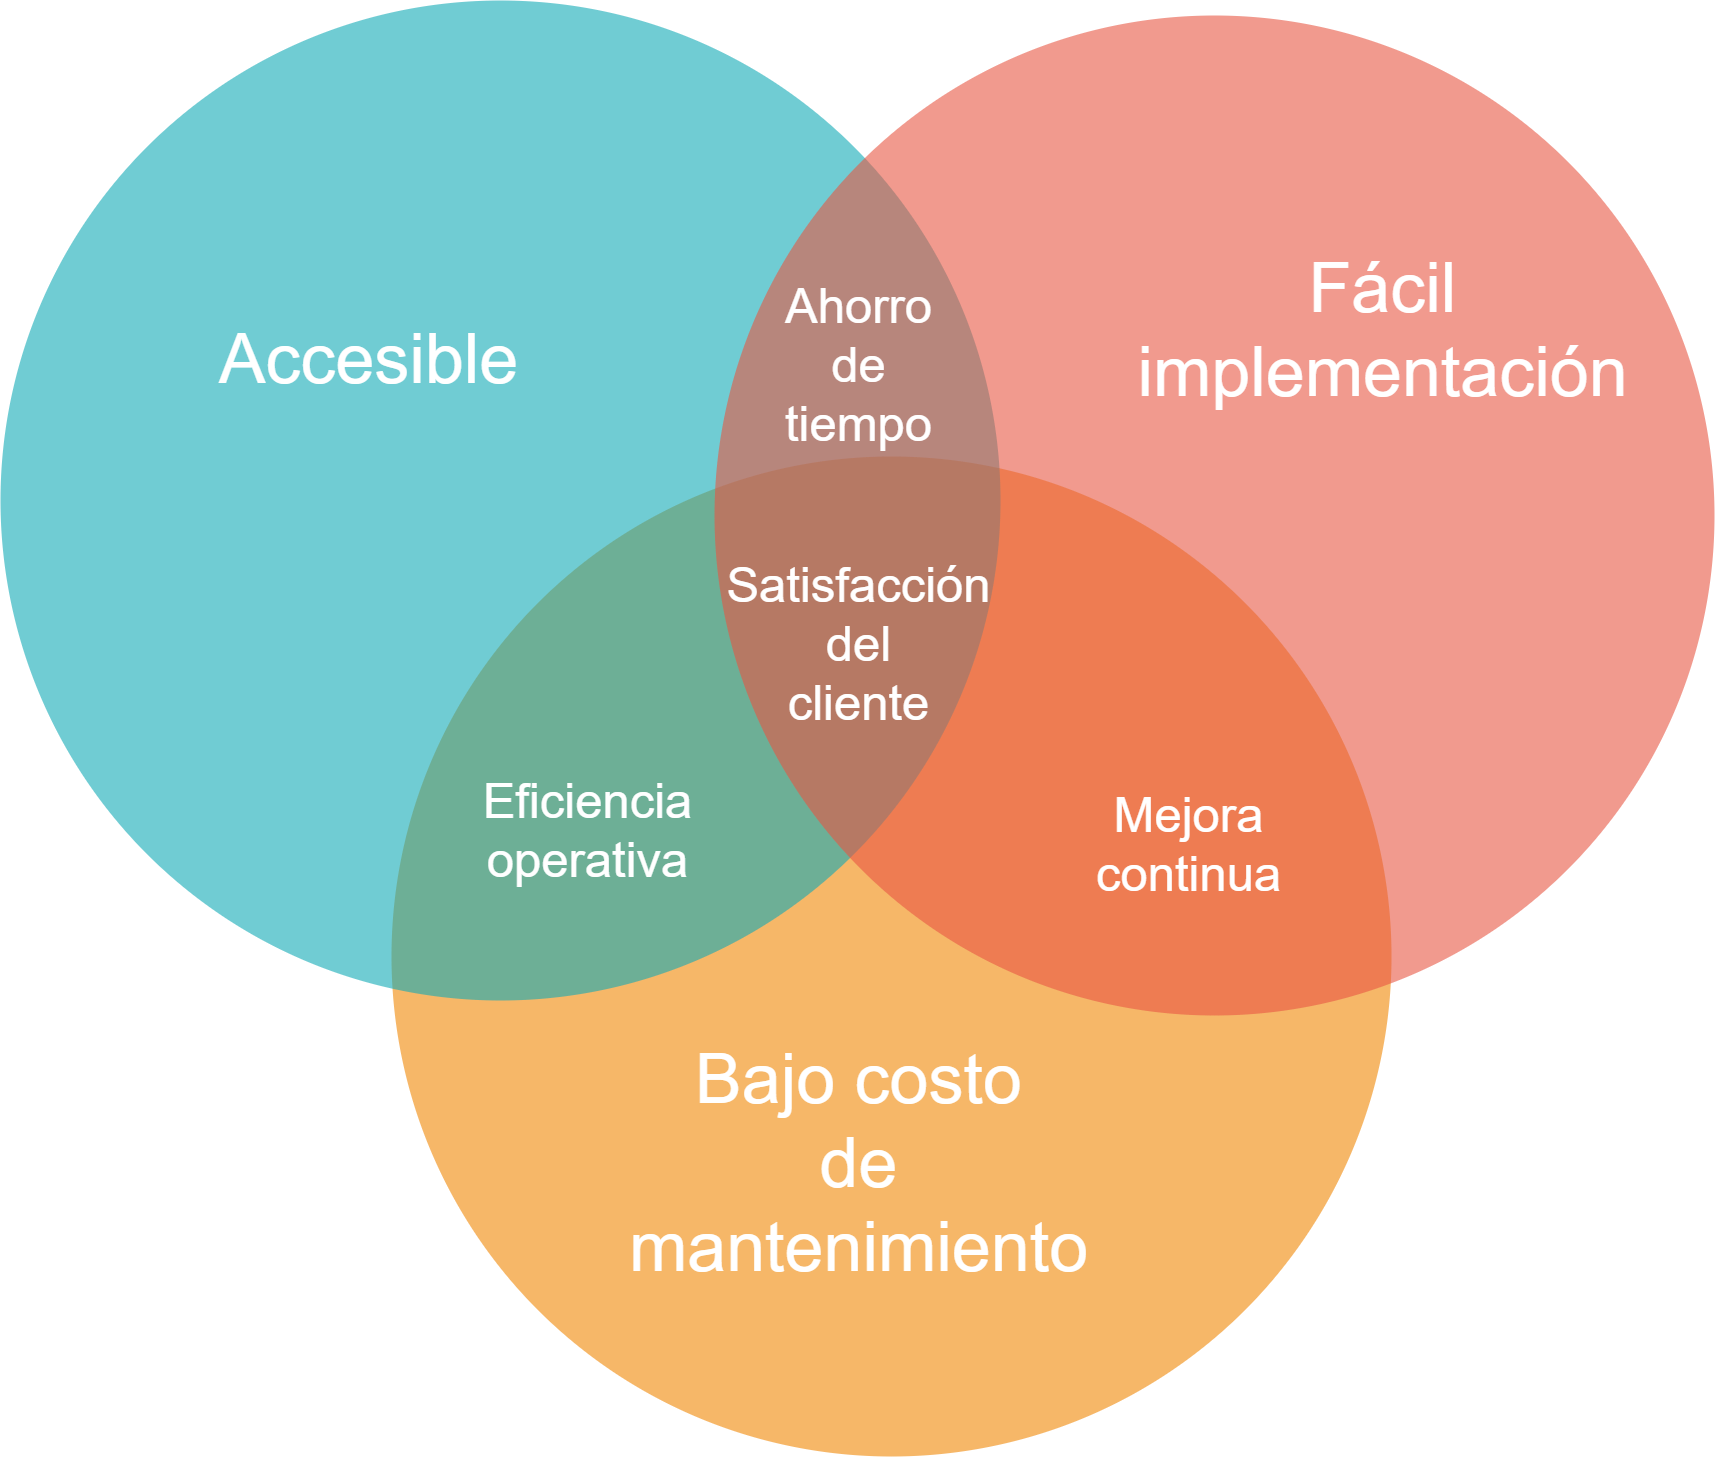
\includegraphics[width=.75\textwidth]{./Figures/Venn_objetivos.png}
  \caption{Relación entre los objetivos centrales.}
  \label{fig:objetivos_venn}
\end{figure}

\subsection{Alcance del trabajo}

Durante la planificación del trabajo se propusieron las siguientes actividades:

\begin{itemize}
    \item Diseño, desarrollo e implementación de un \textit{pipeline} completo para la creación y gestión de chatbots basados en PLN, con capacidad de aprendizaje continuo.
    \item Desarrollo de algoritmos para el preprocesamiento de información y generación de respuestas relevantes y coherentes.
    \item Establecimiento de métricas y procedimientos de evaluación para medir la calidad y eficacia de las respuestas del chatbot.
    \item Implementación de un sistema de retroalimentación que utilice los datos de interacciones con usuarios para mejorar el rendimiento del modelo.
\end{itemize}

Se espera que los resultados incluyan un sistema accesible, de fácil implementación y de bajo costo, que permita a los emprendedores mejorar la eficiencia de sus comunicaciones con los clientes, ahorrando tiempo y mejorando la satisfacción del cliente.



% Si estás familiarizado con \LaTeX{}, entonces podés explorar la estructura de directorios de esta plantilla y proceder a personalizarla agregando tu información en el bloque \emph{INFORMACIÓN DE LA PORTADA} en el archivo \file{memoria.tex}.  

% Se puede continuar luego modificando el resto de los archivos siguiendo los lineamientos que se describen en la sección \ref{sec:FillingFile} en la página \pageref{sec:FillingFile}.

% Debés asegurarte de leer el capítulo \ref{Chapter2} acerca de las convenciones utilizadas para las Memoria de los Trabajos Finales de la \degreename.

% Si sos nuevo en \LaTeX{}, se recomienda que continúes leyendo el documento ya que contiene información básica para aprovechar el potencial de esta herramienta.


%----------------------------------------------------------------------------------------

\section{Estado del arte}
 
\subsection{Revisión de tecnologías}
...
% Esta plantilla se distribuye como una único archivo .zip que se puede descomprimir en varios archivos y carpetas. Asimismo, se puede consultar el repositorio git para obtener la última versión de los archivos, \url{https://github.com/patriciobos/Plantilla-CESE.git}. Los nombres de las carpetas son, o pretender ser, auto-explicativos.

% \keyword{Appendices} -- Esta es la carpeta donde se deben poner los apéndices. Cada apéndice debe ir en su propio archivo \file{.tex}. Se incluye un ejemplo y una plantilla en la carpeta.

% \keyword{Chapters} -- Esta es la carpeta donde se deben poner los capítulos de la memoria. Cada capítulo debe ir un su propio archivo \file{.tex} por separado.  Se ofrece por defecto, la siguiente estructura de capítulos y se recomienda su utilización dentro de lo posible:

% \begin{itemize}
% \item Capítulo 1: Introducción general	
% \item Capítulo 2: Introducción específica
% \item Capítulo 3: Diseño e implementación
% \item Capítulo 4: Ensayos y resultados
% \item Capítulo 5: Conclusiones

% \end{itemize}

% Esta estructura de capítulos es la que se recomienda para las memorias de la especialización.

% \keyword{Figures} -- Esta carpeta contiene todas las figuras de la memoria.  Estas son las versiones finales de las imágenes que van a ser incluidas en la memoria.  Pueden ser imágenes en formato \textit{raster}\footnote{\url{https://en.wikipedia.org/wiki/Raster_graphics}} como \file{.png}, \file{.jpg} o en formato vectoriales\footnote{\url{https://en.wikipedia.org/wiki/Vector_graphics}} como \file{.pdf}, \file{.ps}.  Se debe notar que utilizar imágenes vectoriales disminuye notablemente el peso del documento final y acelera el tiempo de compilación por lo que es recomendable su utilización siempre que sea posible.

\subsection{investigaciones previas y tendencias actuales}

...
% También están incluidos varios archivos, la mayoría de ellos son de texto plano y se puede ver su contenido en un editor de texto. Después de la compilación inicial, se verá que más archivos auxiliares son creados por \ LaTeX{} o BibTeX, pero son de uso interno y no es necesario hacer nada en particular con ellos.  Toda la información necesaria para compilar el documento se encuentra en los archivos \file{.tex}, \file{.bib}, \file{.cls} y en las imágenes de la carpeta Figures.

% \keyword{referencias.bib} - este es un archivo importante que contiene toda la información de referencias bibliográficas que se utilizarán para las citas en la memoria en conjunto con BibTeX. Usted puede escribir las entradas bibliográficas en forma manual, aunque existen también programas de gestión de referencias que facilitan la creación y gestión de las referencias y permiten exportarlas en formato BibTeX.  También hay disponibles sitios web como \url{books.google.com} que permiten obtener toda la información necesaria para una cita en formato BibTeX. Ver sección \ref{sec:biblio}

% \keyword{MastersDoctoralThesis.cls} -- este es un archivo importante. Es el archivos con la clase que le informa a \LaTeX{} cómo debe dar formato a la memoria. El usuario de la plantilla no debería necesitar modificar nada de este archivo.

% \keyword{memoria.pdf} -- esta es su memoria con una tipografía bellamente compuesta (en formato de archivo PDF) creado por \LaTeX{}. Se distribuye con la plantilla y después de compilar por primera vez sin hacer ningún cambio se debería obtener una versión idéntica a este documento.

% \keyword{memoria.tex} -- este es un archivo importante. Este es el archivo que tiene que compilar \LaTeX{} para producir la memoria como un archivo PDF. Contiene un marco de trabajo y estructuras que le indican a \LaTeX{} cómo diagramar la memoria.  Está altamente comentado para que se pueda entender qué es lo que realiza cada línea de código y por qué está incluida en ese lugar.  En este archivo se debe completar la información personalizada de las primeras sección según se indica en la sección \ref{sec:FillingFile}.

% Archivos que \emph{no} forman parte de la distribución de la plantilla pero que son generados por \LaTeX{} como archivos auxiliares necesarios para la producción de la memoria.pdf son:

% \keyword{memoria.aux} -- este es un archivo auxiliar generado por \LaTeX{}, si se borra \LaTeX{} simplemente lo regenera cuando se compila el archivo principal \file{memoria.tex}.

% \keyword{memoria.bbl} -- este es un archivo auxiliar generado por BibTeX, si se borra BibTeX simplemente lo regenera cuando se compila el archivo principal \file{memoria.tex}. Mientras que el archivo \file{.bib} contiene todas las referencias que hay, este archivo \file{.bbl} contine sólo las referencias que han sido citadas y se utiliza para la construcción de la bibiografía.

% \keyword{memoria.blg} -- este es un archivo auxiliar generado por BibTeX, si se borra BibTeX simplemente lo regenera cuando se compila el archivo principal \file{memoria.tex}.

% \keyword{memoria.lof} -- este es un archivo auxiliar generado por \LaTeX{}, si se borra \LaTeX{} simplemente lo regenera cuando se compila el archivo principal \file{memoria.tex}.  Le indica a \LaTeX{} cómo construir la sección \emph{Lista de Figuras}.
 
% \keyword{memoria.log} --  este es un archivo auxiliar generado por \LaTeX{}, si se borra \LaTeX{} simplemente lo regenera cuando se compila el archivo principal \file{memoria.tex}. Contiene mensajes de \LaTeX{}. Si se reciben errores o advertencias durante la compilación, se guardan en este archivo \file{.log}.

% \keyword{memoria.lot} -- este es un archivo auxiliar generado por \LaTeX{}, si se borra \LaTeX{} simplemente lo regenera cuando se compila el archivo principal \file{memoria.tex}.  Le indica a \LaTeX{} cómo construir la sección \emph{Lista de Tablas}.

% \keyword{memoria.out} -- este es un archivo auxiliar generado por \LaTeX{}, si se borra \LaTeX{} simplemente lo regenera cuando se compila el archivo principal \file{memoria.tex}.

% De esta larga lista de archivos, sólo aquellos con la extensión \file{.bib}, \file{.cls} y \file{.tex} son importantes.  Los otros archivos auxiliares pueden ser ignorados o borrados ya que \LaTeX{} y BibTeX los regenerarán durante la compilación.

%----------------------------------------------------------------------------------------

% \section{Entorno de trabajo}

% Ante de comenzar a editar la plantilla debemos tener un editor \LaTeX{} instalado en nuestra computadora.  En forma análoga a lo que sucede en lenguaje C, que se puede crear y editar código con casi cualquier editor, existen ciertos entornos de trabajo que nos pueden simplificar mucho la tarea.  En este sentido, se recomienda, sobre todo para los principiantes en \LaTeX{} la utilización de TexMaker, un programa gratuito y multi-plantaforma que está disponible tanto para windows como para sistemas GNU/linux.

% La versión más reciente de TexMaker es la 4.5 y se puede descargar del siguiente link: \url{http://www.xm1math.net/texmaker/download.html}. Se puede consultar el manual de usuario en el siguiente link: \url{http://www.xm1math.net/texmaker/doc.html}.
 

% \subsection{Paquetes adicionales}

% Si bien durante el proceso de instalación de TexMaker, o cualquier otro editor que se haya elegido, se instalarán en el sistema los paquetes básicos necesarios para trabajar con \LaTeX{}, la plantilla de los trabajos de Especialización y Maestría requieren de paquete adicionales.

% Se indican a continuación los comandos que se deben introducir en la consola de Ubuntu (ctrl + alt + t) para instalarlos:

% \begin{lstlisting}[language=bash]
%   $ sudo apt install texlive-lang-spanish texlive-science 
%   $ sudo apt install texlive-bibtex-extra biber
%   $ sudo apt install texlive texlive-fonts-recommended
%   $ sudo apt install texlive-latex-extra
% \end{lstlisting}


% \subsection{Configurando TexMaker}
% \label{subsec:configurando}



% Una vez instalado el programa y los paquetes adicionales se debe abrir el archivo memoria.tex con el editor para ver una pantalla similar a la que se puede apreciar en la figura \ref{fig:texmaker}. 
% Una vez instalado el programa y los paquetes adicionales se debe abrir el archivo memoria.tex con el editor para ver una pantalla similar a la que se puede apreciar en la figura \ref{fig:texmaker}. 
% Una vez instalado el programa y los paquetes adicionales se debe abrir el archivo memoria.tex con el editor para ver una pantalla similar a la que se puede apreciar en la figura \ref{fig:texmaker}. 
% Una vez instalado el programa y los paquetes adicionales se debe abrir el archivo memoria.tex con el editor para ver una pantalla similar a la que se puede apreciar en la figura \ref{fig:texmaker}. 

% \vspace{1cm}

% \begin{figure}[htbp]
% 	\centering
% 	\includegraphics[width=.5\textwidth]{./Figures/texmaker.png}
% 	\caption{Entorno de trabajo de texMaker.}
% 	\label{fig:texmaker}
% \end{figure}

% \vspace{1cm}

% Notar que existe una vista llamada Estructura a la izquierda de la interfaz que nos permite abrir desde dentro del programa los archivos individuales de los capítulos.  A la derecha se encuentra una vista con el archivo propiamente dicho para su edición. Hacia la parte inferior se encuentra una vista del log con información de los resultados de la compilación.  En esta última vista pueden aparecen advertencias o \textit{warning}, que normalmente pueden ser ignorados, y los errores que se indican en color rojo y deben resolverse para que se genere el PDF de salida.

% Recordar que el archivo que se debe compilar con PDFLaTeX es \file{memoria.tex}, si se tratara de compilar alguno de los capítulos saldría un error.  Para salvar la molestia de tener que cambiar de archivo para compilar cada vez que se realice una modificación en un capítulo, se puede definir el archivo \file{memoria.tex} como ``documento maestro'' yendo al menú opciones -> ``definir documento actual como documento maestro'', lo que permite compilar con PDFLaTeX memoria.tex directamente desde cualquier archivo que se esté modificando . Se muestra esta opción en la figura \ref{fig:docMaestro}.

% \begin{figure}[h]
% 	\centering
% 	\includegraphics[width=\textwidth]{./Figures/docMaestro.png}
% 	\caption{Definir memoria.tex como documento maestro.}
% 	\label{fig:docMaestro}
% \end{figure}

% En el menú herramientas se encuentran las opciones de compilación.  Para producir un archivo PDF a partir de un archivo .tex se debe ejecutar PDFLaTeX (el shortcut es F6). Para incorporar nueva bibliografía se debe utilizar la opción BibTeX del mismo menú herramientas (el shortcut es F11).

% Notar que para actualizar las tablas de contenidos se debe ejecutar PDFLaTeX dos veces.  Esto se debe a que es necesario actualizar algunos archivos auxiliares antes de obtener el resultado final.  En forma similar, para actualizar las referencias bibliográficas se debe ejecutar primero PDFLaTeX, después BibTeX y finalmente PDFLaTeX dos veces por idénticos motivos.

% \section{Personalizando la plantilla, el archivo \file{memoria.tex}}
% \label{sec:FillingFile}

% Para personalizar la plantilla se debe incorporar la información propia en los distintos archivos \file{.tex}. 

% Primero abrir \file{memoria.tex} con TexMaker (o el editor de su preferencia). Se debe ubicar dentro del archivo el bloque de código titulado \emph{INFORMACIÓN DE LA PORTADA} donde se deben incorporar los primeros datos personales con los que se construirá automáticamente la portada.


% %----------------------------------------------------------------------------------------

% \section{El código del archivo \file{memoria.tex} explicado}

% El archivo \file{memoria.tex} contiene la estructura del documento y es el archivo de mayor jerarquía de la memoria.  Podría ser equiparable a la función \emph{main()} de un programa en C, o mejor dicho al archivo fuente .c donde se encuentra definida la función main().

% La estructura básica de cualquier documento de \LaTeX{} comienza con la definición de clase del documento, es seguida por un preámbulo donde se pueden agregar funcionalidades con el uso de \texttt{paquetes} (equiparables a bibliotecas de C), y finalmente, termina con el cuerpo del documento, donde irá el contenido de la memoria.

% \lstset{%
%   basicstyle=\small\ttfamily,
%   language=[LaTeX]{TeX}
% }

% \begin{lstlisting}
% \documentclass{article}  <- Definicion de clase
% \usepackage{listings}	 <- Preambulo

% \begin{document}	 <- Comienzo del contenido propio 
% 	Hello world!
% \end{document}
% \end{lstlisting}


% El archivo \file{memoria.tex} se encuentra densamente comentado para explicar qué páginas, secciones y elementos de formato está creando el código \LaTeX{} en cada línea. El código está dividido en bloques con nombres en mayúsculas para que resulte evidente qué es lo que hace esa porción de código en particular. Inicialmente puede parecer que hay mucho código \LaTeX{}, pero es principalmente código para dar formato a la memoria por lo que no requiere intervención del usuario de la plantilla.  Sí se deben personalizar con su información los bloques indicados como:

% \begin{itemize}
% 	\item Informacion de la memoria
% 	\item Resumen
% 	\item Agradecimientos
% 	\item Dedicatoria
% \end{itemize}

% El índice de contenidos, las listas de figura de tablas se generan en forma automática y no requieren intervención ni edición manual por parte del usuario de la plantilla. 

% En la parte final del documento se encuentran los capítulos y los apéndices.  Por defecto se incluyen los 5 capítulos propuestos que se encuentran en la carpeta /Chapters. Cada capítulo se debe escribir en un archivo .tex separado y se debe poner en la carpeta \emph{Chapters} con el nombre \file{Chapter1}, \file{Chapter2}, etc\ldots El código para incluir capítulos desde archivos externos se muestra a continuación.

% \begin{verbatim}
% 	% Chapter 1

\chapter{Introducción general} % Main chapter title

\label{Chapter1} % For referencing the chapter elsewhere, use \ref{Chapter1} 
\label{IntroGeneral}


%----------------------------------------------------------------------------------------

% Define some commands to keep the formatting separated from the content 
\newcommand{\keyword}[1]{\textbf{#1}}
\newcommand{\tabhead}[1]{\textbf{#1}}
\newcommand{\code}[1]{\texttt{#1}}
\newcommand{\file}[1]{\texttt{\bfseries#1}}
\newcommand{\option}[1]{\texttt{\itshape#1}}
\newcommand{\grados}{$^{\circ}$}

%----------------------------------------------------------------------------------------

%\section{Introducción}

%----------------------------------------------------------------------------------------
% \section{Resumen inicial{}}
En este capítulo se exploran las motivaciones que impulsaron el desarrollo del sistema, diseñado para automatizar la comunicación entre emprendedores y sus clientes. Se ofrece, además, una explicación detallada sobre qué son los chatbots y las razones por las que su uso resulta fundamental en este contexto. Finalmente, se describen los objetivos principales del trabajo, centrados en la facilidad de implementación y en la mejora de la eficiencia operativa, junto con el alcance definido durante la planificación.

\section{Motivación{}}

El sistema desarrollado en el presente trabajo surge de la necesidad de proporcionar a emprendedores una herramienta que les permita automatizar la comunicación con sus clientes de manera eficiente y personalizada. Esta herramienta les ofrece una ventaja competitiva al optimizar la gestión de sus interacciones con los usuarios y les permite mejorar la eficiencia operativa, además de reducir los costos asociados a la atención al cliente.


\subsection{¿Qué es un chatbot?}

Un chatbot es un programa de software que emplea técnicas de Procesamiento del Lenguaje Natural (PLN)\footnote{El procesamiento de lenguaje natural, o PLN, combina la lingüística computacional (modelado del lenguaje humano basado en reglas) con modelos estadísticos y de aprendizaje automático para permitir que las computadoras y los dispositivos digitales reconozcan, comprendan y generen texto y voz. \url{https://www.ibm.com/mx-es/topics/natural-language-processing}} para interpretar y contestar automáticamente las consultas de los usuarios de manera coherente y eficiente. Esto facilita la automatización de interacciones comunes y mejora la experiencia del cliente.

\subsubsection{¿Por qué un chatbot?}

A continuación, se destacan algunas de las razones principales por las cuales un chatbot es la solución ideal para este trabajo:

\begin{itemize}
    \item Disponibilidad 24/7: los chatbots están disponibles en todo momento, lo que permite a las empresas atender consultas de sus clientes a cualquier hora del día.
    
    \item Reducción de costos: al automatizar la atención al cliente, los chatbots permiten a las empresas reducir los costos asociados a personal humano, sin comprometer la calidad del servicio.
    
    \item Recolección de datos valiosos: los chatbots pueden recopilar y analizar información relevante sobre las interacciones con los clientes, lo que permite a las empresas ajustar sus estrategias de manera eficiente.
    
    \item Optimización de tiempos de respuesta: la capacidad de generar respuestas inmediatas en función de consultas predefinidas optimiza los tiempos de respuesta.
\end{itemize}

% \subsection{Guía matemática rápida para \LaTeX{}}

% Si estás escribiendo un documento con mucho contenido matemático, entonces es posible que desees leer el documento de la AMS (American Mathematical Society) llamado, \enquote{A Short Math Guide for \LaTeX{}}. Se puede encontrar en línea en el siguiente link: \url{http://www.ams.org/tex/amslatex.html} en la sección \enquote{Additional Documentation} hacia la parte inferior de la página.


%----------------------------------------------------------------------------------------
% \newpage % agrego un salto de página 
\subsection{Objetivos principales}

El trabajo se enfoca en tres objetivos principales que se interrelacionan para ofrecer una solución integral a pequeños emprendedores. Cada uno de estos objetivos está orientado a asegurar que la herramienta sea accesible, fácilmente implementable y de bajo costo, para garantizar una experiencia eficiente y optimizada para las empresas que la adopten. 
 
A continuación, se detallan los objetivos principales:


\begin{itemize}
    \item Hacer accesible la solución a pequeños emprendedores: desarrollar un sistema que sea de fácil adopción y pueda ser utilizado por pequeñas empresas, independientemente de sus conocimientos técnicos.
    
    \item Garantizar una fácil implementación: diseñar una solución replicable, de manera que cualquier empresa pueda contar con el chatbot simplemente proporcionando el contexto necesario para su entrenamiento. No será necesario disponer de infraestructura compleja ni personal especializado.
    
    \item Reducir el costo de mantenimiento: proporcionar una herramienta con un bajo costo de mantenimiento, tanto en términos económicos como de tiempo, para que los emprendedores puedan centrarse en su negocio principal.
    
\end{itemize}


% Incluir aquí el gráfico de Venn que detalle la relación de los objetivos principales.
% \includegraphics[width=\textwidth]{ruta/al/grafico_venn.png}

\begin{figure}[htbp]

  \centering
  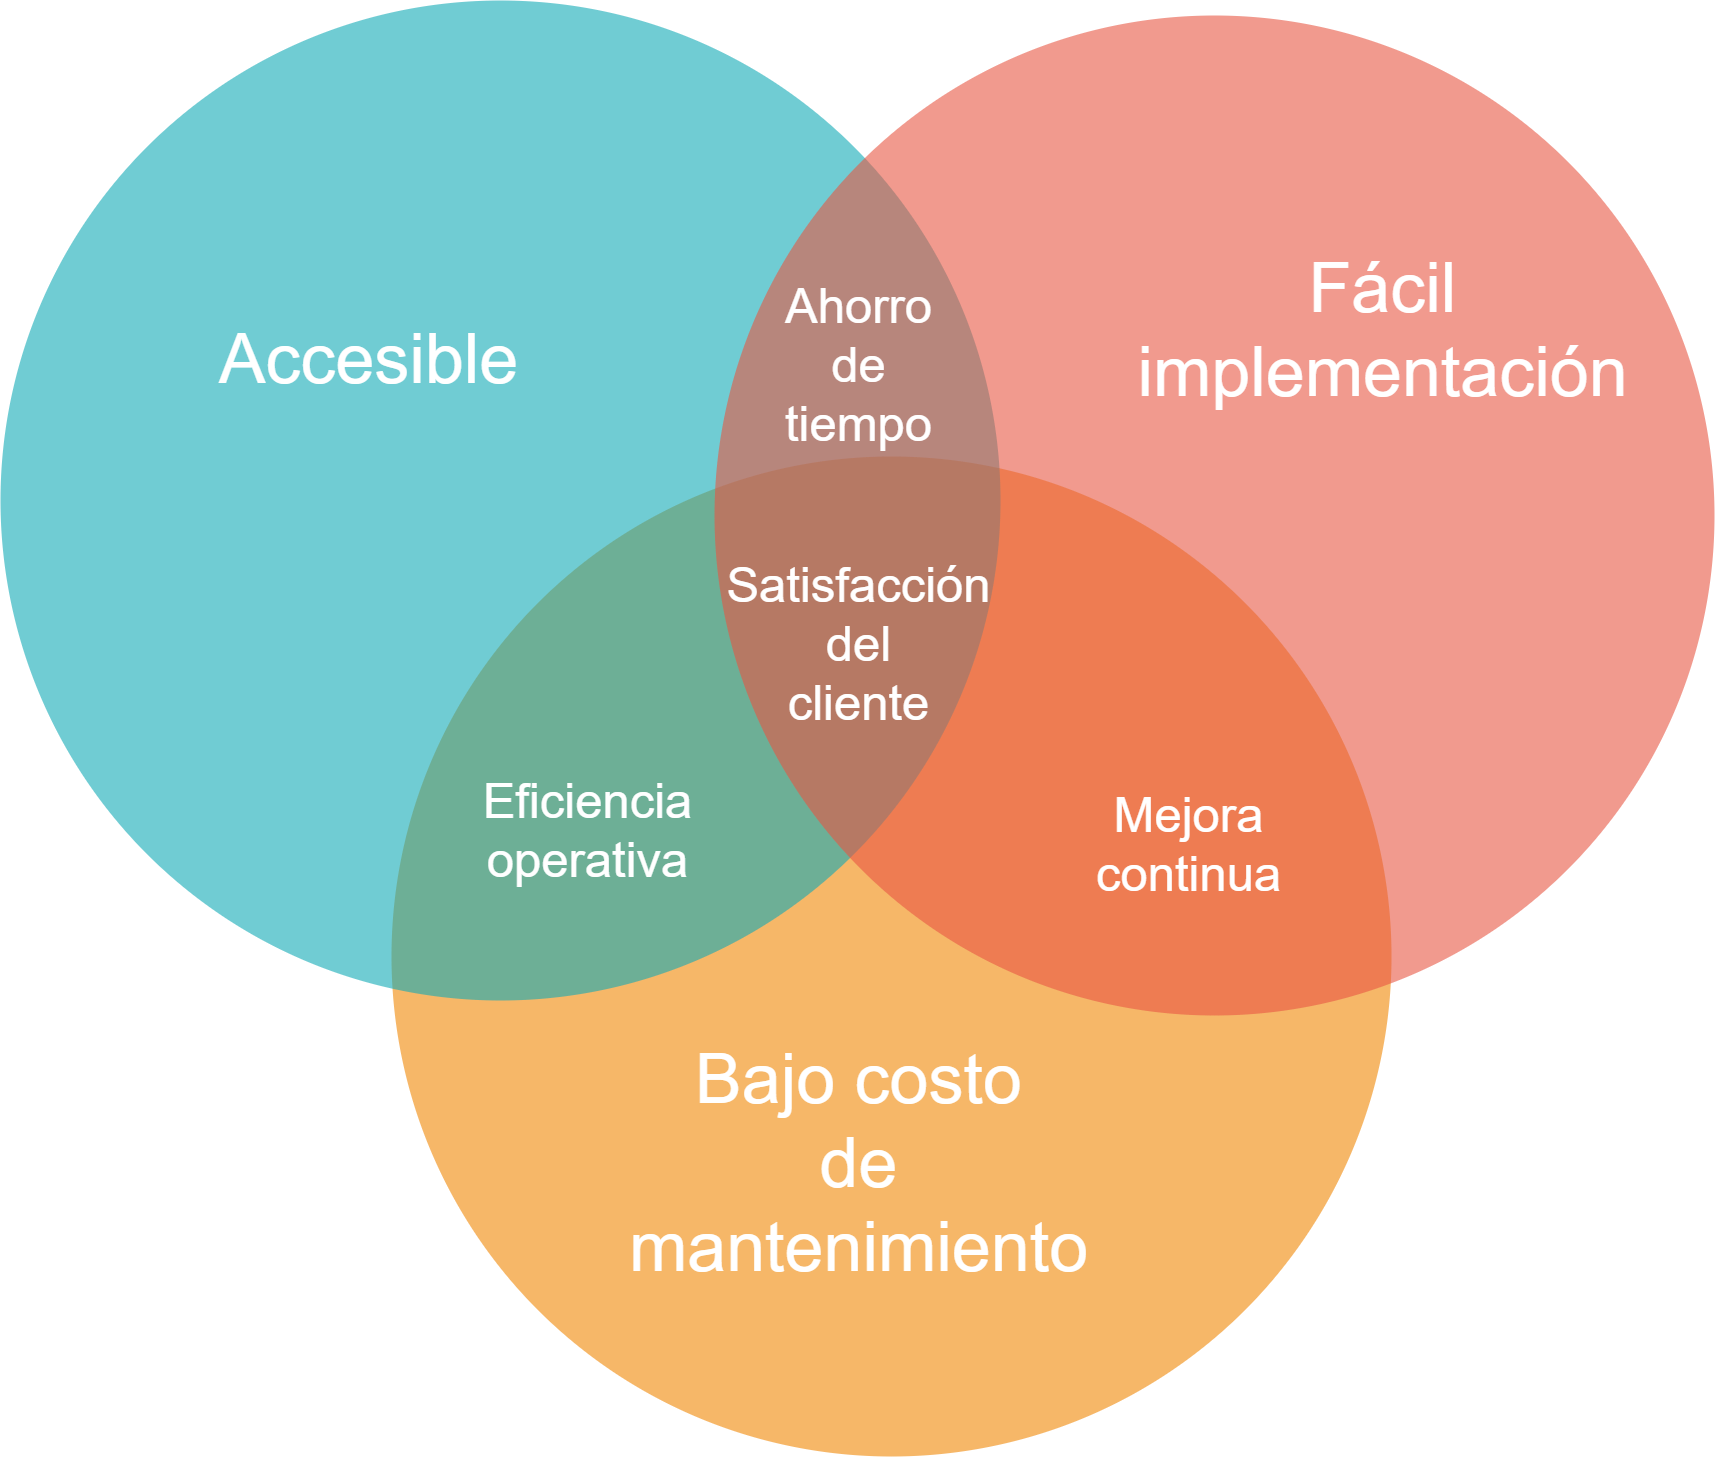
\includegraphics[width=.75\textwidth]{./Figures/Venn_objetivos.png}
  \caption{Relación entre los objetivos centrales.}
  \label{fig:objetivos_venn}
\end{figure}

\subsection{Alcance del trabajo}

Durante la planificación del trabajo se propusieron las siguientes actividades:

\begin{itemize}
    \item Diseño, desarrollo e implementación de un \textit{pipeline} completo para la creación y gestión de chatbots basados en PLN, con capacidad de aprendizaje continuo.
    \item Desarrollo de algoritmos para el preprocesamiento de información y generación de respuestas relevantes y coherentes.
    \item Establecimiento de métricas y procedimientos de evaluación para medir la calidad y eficacia de las respuestas del chatbot.
    \item Implementación de un sistema de retroalimentación que utilice los datos de interacciones con usuarios para mejorar el rendimiento del modelo.
\end{itemize}

Se espera que los resultados incluyan un sistema accesible, de fácil implementación y de bajo costo, que permita a los emprendedores mejorar la eficiencia de sus comunicaciones con los clientes, ahorrando tiempo y mejorando la satisfacción del cliente.



% Si estás familiarizado con \LaTeX{}, entonces podés explorar la estructura de directorios de esta plantilla y proceder a personalizarla agregando tu información en el bloque \emph{INFORMACIÓN DE LA PORTADA} en el archivo \file{memoria.tex}.  

% Se puede continuar luego modificando el resto de los archivos siguiendo los lineamientos que se describen en la sección \ref{sec:FillingFile} en la página \pageref{sec:FillingFile}.

% Debés asegurarte de leer el capítulo \ref{Chapter2} acerca de las convenciones utilizadas para las Memoria de los Trabajos Finales de la \degreename.

% Si sos nuevo en \LaTeX{}, se recomienda que continúes leyendo el documento ya que contiene información básica para aprovechar el potencial de esta herramienta.


%----------------------------------------------------------------------------------------

\section{Estado del arte}
 
\subsection{Revisión de tecnologías}
...
% Esta plantilla se distribuye como una único archivo .zip que se puede descomprimir en varios archivos y carpetas. Asimismo, se puede consultar el repositorio git para obtener la última versión de los archivos, \url{https://github.com/patriciobos/Plantilla-CESE.git}. Los nombres de las carpetas son, o pretender ser, auto-explicativos.

% \keyword{Appendices} -- Esta es la carpeta donde se deben poner los apéndices. Cada apéndice debe ir en su propio archivo \file{.tex}. Se incluye un ejemplo y una plantilla en la carpeta.

% \keyword{Chapters} -- Esta es la carpeta donde se deben poner los capítulos de la memoria. Cada capítulo debe ir un su propio archivo \file{.tex} por separado.  Se ofrece por defecto, la siguiente estructura de capítulos y se recomienda su utilización dentro de lo posible:

% \begin{itemize}
% \item Capítulo 1: Introducción general	
% \item Capítulo 2: Introducción específica
% \item Capítulo 3: Diseño e implementación
% \item Capítulo 4: Ensayos y resultados
% \item Capítulo 5: Conclusiones

% \end{itemize}

% Esta estructura de capítulos es la que se recomienda para las memorias de la especialización.

% \keyword{Figures} -- Esta carpeta contiene todas las figuras de la memoria.  Estas son las versiones finales de las imágenes que van a ser incluidas en la memoria.  Pueden ser imágenes en formato \textit{raster}\footnote{\url{https://en.wikipedia.org/wiki/Raster_graphics}} como \file{.png}, \file{.jpg} o en formato vectoriales\footnote{\url{https://en.wikipedia.org/wiki/Vector_graphics}} como \file{.pdf}, \file{.ps}.  Se debe notar que utilizar imágenes vectoriales disminuye notablemente el peso del documento final y acelera el tiempo de compilación por lo que es recomendable su utilización siempre que sea posible.

\subsection{investigaciones previas y tendencias actuales}

...
% También están incluidos varios archivos, la mayoría de ellos son de texto plano y se puede ver su contenido en un editor de texto. Después de la compilación inicial, se verá que más archivos auxiliares son creados por \ LaTeX{} o BibTeX, pero son de uso interno y no es necesario hacer nada en particular con ellos.  Toda la información necesaria para compilar el documento se encuentra en los archivos \file{.tex}, \file{.bib}, \file{.cls} y en las imágenes de la carpeta Figures.

% \keyword{referencias.bib} - este es un archivo importante que contiene toda la información de referencias bibliográficas que se utilizarán para las citas en la memoria en conjunto con BibTeX. Usted puede escribir las entradas bibliográficas en forma manual, aunque existen también programas de gestión de referencias que facilitan la creación y gestión de las referencias y permiten exportarlas en formato BibTeX.  También hay disponibles sitios web como \url{books.google.com} que permiten obtener toda la información necesaria para una cita en formato BibTeX. Ver sección \ref{sec:biblio}

% \keyword{MastersDoctoralThesis.cls} -- este es un archivo importante. Es el archivos con la clase que le informa a \LaTeX{} cómo debe dar formato a la memoria. El usuario de la plantilla no debería necesitar modificar nada de este archivo.

% \keyword{memoria.pdf} -- esta es su memoria con una tipografía bellamente compuesta (en formato de archivo PDF) creado por \LaTeX{}. Se distribuye con la plantilla y después de compilar por primera vez sin hacer ningún cambio se debería obtener una versión idéntica a este documento.

% \keyword{memoria.tex} -- este es un archivo importante. Este es el archivo que tiene que compilar \LaTeX{} para producir la memoria como un archivo PDF. Contiene un marco de trabajo y estructuras que le indican a \LaTeX{} cómo diagramar la memoria.  Está altamente comentado para que se pueda entender qué es lo que realiza cada línea de código y por qué está incluida en ese lugar.  En este archivo se debe completar la información personalizada de las primeras sección según se indica en la sección \ref{sec:FillingFile}.

% Archivos que \emph{no} forman parte de la distribución de la plantilla pero que son generados por \LaTeX{} como archivos auxiliares necesarios para la producción de la memoria.pdf son:

% \keyword{memoria.aux} -- este es un archivo auxiliar generado por \LaTeX{}, si se borra \LaTeX{} simplemente lo regenera cuando se compila el archivo principal \file{memoria.tex}.

% \keyword{memoria.bbl} -- este es un archivo auxiliar generado por BibTeX, si se borra BibTeX simplemente lo regenera cuando se compila el archivo principal \file{memoria.tex}. Mientras que el archivo \file{.bib} contiene todas las referencias que hay, este archivo \file{.bbl} contine sólo las referencias que han sido citadas y se utiliza para la construcción de la bibiografía.

% \keyword{memoria.blg} -- este es un archivo auxiliar generado por BibTeX, si se borra BibTeX simplemente lo regenera cuando se compila el archivo principal \file{memoria.tex}.

% \keyword{memoria.lof} -- este es un archivo auxiliar generado por \LaTeX{}, si se borra \LaTeX{} simplemente lo regenera cuando se compila el archivo principal \file{memoria.tex}.  Le indica a \LaTeX{} cómo construir la sección \emph{Lista de Figuras}.
 
% \keyword{memoria.log} --  este es un archivo auxiliar generado por \LaTeX{}, si se borra \LaTeX{} simplemente lo regenera cuando se compila el archivo principal \file{memoria.tex}. Contiene mensajes de \LaTeX{}. Si se reciben errores o advertencias durante la compilación, se guardan en este archivo \file{.log}.

% \keyword{memoria.lot} -- este es un archivo auxiliar generado por \LaTeX{}, si se borra \LaTeX{} simplemente lo regenera cuando se compila el archivo principal \file{memoria.tex}.  Le indica a \LaTeX{} cómo construir la sección \emph{Lista de Tablas}.

% \keyword{memoria.out} -- este es un archivo auxiliar generado por \LaTeX{}, si se borra \LaTeX{} simplemente lo regenera cuando se compila el archivo principal \file{memoria.tex}.

% De esta larga lista de archivos, sólo aquellos con la extensión \file{.bib}, \file{.cls} y \file{.tex} son importantes.  Los otros archivos auxiliares pueden ser ignorados o borrados ya que \LaTeX{} y BibTeX los regenerarán durante la compilación.

%----------------------------------------------------------------------------------------

% \section{Entorno de trabajo}

% Ante de comenzar a editar la plantilla debemos tener un editor \LaTeX{} instalado en nuestra computadora.  En forma análoga a lo que sucede en lenguaje C, que se puede crear y editar código con casi cualquier editor, existen ciertos entornos de trabajo que nos pueden simplificar mucho la tarea.  En este sentido, se recomienda, sobre todo para los principiantes en \LaTeX{} la utilización de TexMaker, un programa gratuito y multi-plantaforma que está disponible tanto para windows como para sistemas GNU/linux.

% La versión más reciente de TexMaker es la 4.5 y se puede descargar del siguiente link: \url{http://www.xm1math.net/texmaker/download.html}. Se puede consultar el manual de usuario en el siguiente link: \url{http://www.xm1math.net/texmaker/doc.html}.
 

% \subsection{Paquetes adicionales}

% Si bien durante el proceso de instalación de TexMaker, o cualquier otro editor que se haya elegido, se instalarán en el sistema los paquetes básicos necesarios para trabajar con \LaTeX{}, la plantilla de los trabajos de Especialización y Maestría requieren de paquete adicionales.

% Se indican a continuación los comandos que se deben introducir en la consola de Ubuntu (ctrl + alt + t) para instalarlos:

% \begin{lstlisting}[language=bash]
%   $ sudo apt install texlive-lang-spanish texlive-science 
%   $ sudo apt install texlive-bibtex-extra biber
%   $ sudo apt install texlive texlive-fonts-recommended
%   $ sudo apt install texlive-latex-extra
% \end{lstlisting}


% \subsection{Configurando TexMaker}
% \label{subsec:configurando}



% Una vez instalado el programa y los paquetes adicionales se debe abrir el archivo memoria.tex con el editor para ver una pantalla similar a la que se puede apreciar en la figura \ref{fig:texmaker}. 
% Una vez instalado el programa y los paquetes adicionales se debe abrir el archivo memoria.tex con el editor para ver una pantalla similar a la que se puede apreciar en la figura \ref{fig:texmaker}. 
% Una vez instalado el programa y los paquetes adicionales se debe abrir el archivo memoria.tex con el editor para ver una pantalla similar a la que se puede apreciar en la figura \ref{fig:texmaker}. 
% Una vez instalado el programa y los paquetes adicionales se debe abrir el archivo memoria.tex con el editor para ver una pantalla similar a la que se puede apreciar en la figura \ref{fig:texmaker}. 

% \vspace{1cm}

% \begin{figure}[htbp]
% 	\centering
% 	\includegraphics[width=.5\textwidth]{./Figures/texmaker.png}
% 	\caption{Entorno de trabajo de texMaker.}
% 	\label{fig:texmaker}
% \end{figure}

% \vspace{1cm}

% Notar que existe una vista llamada Estructura a la izquierda de la interfaz que nos permite abrir desde dentro del programa los archivos individuales de los capítulos.  A la derecha se encuentra una vista con el archivo propiamente dicho para su edición. Hacia la parte inferior se encuentra una vista del log con información de los resultados de la compilación.  En esta última vista pueden aparecen advertencias o \textit{warning}, que normalmente pueden ser ignorados, y los errores que se indican en color rojo y deben resolverse para que se genere el PDF de salida.

% Recordar que el archivo que se debe compilar con PDFLaTeX es \file{memoria.tex}, si se tratara de compilar alguno de los capítulos saldría un error.  Para salvar la molestia de tener que cambiar de archivo para compilar cada vez que se realice una modificación en un capítulo, se puede definir el archivo \file{memoria.tex} como ``documento maestro'' yendo al menú opciones -> ``definir documento actual como documento maestro'', lo que permite compilar con PDFLaTeX memoria.tex directamente desde cualquier archivo que se esté modificando . Se muestra esta opción en la figura \ref{fig:docMaestro}.

% \begin{figure}[h]
% 	\centering
% 	\includegraphics[width=\textwidth]{./Figures/docMaestro.png}
% 	\caption{Definir memoria.tex como documento maestro.}
% 	\label{fig:docMaestro}
% \end{figure}

% En el menú herramientas se encuentran las opciones de compilación.  Para producir un archivo PDF a partir de un archivo .tex se debe ejecutar PDFLaTeX (el shortcut es F6). Para incorporar nueva bibliografía se debe utilizar la opción BibTeX del mismo menú herramientas (el shortcut es F11).

% Notar que para actualizar las tablas de contenidos se debe ejecutar PDFLaTeX dos veces.  Esto se debe a que es necesario actualizar algunos archivos auxiliares antes de obtener el resultado final.  En forma similar, para actualizar las referencias bibliográficas se debe ejecutar primero PDFLaTeX, después BibTeX y finalmente PDFLaTeX dos veces por idénticos motivos.

% \section{Personalizando la plantilla, el archivo \file{memoria.tex}}
% \label{sec:FillingFile}

% Para personalizar la plantilla se debe incorporar la información propia en los distintos archivos \file{.tex}. 

% Primero abrir \file{memoria.tex} con TexMaker (o el editor de su preferencia). Se debe ubicar dentro del archivo el bloque de código titulado \emph{INFORMACIÓN DE LA PORTADA} donde se deben incorporar los primeros datos personales con los que se construirá automáticamente la portada.


% %----------------------------------------------------------------------------------------

% \section{El código del archivo \file{memoria.tex} explicado}

% El archivo \file{memoria.tex} contiene la estructura del documento y es el archivo de mayor jerarquía de la memoria.  Podría ser equiparable a la función \emph{main()} de un programa en C, o mejor dicho al archivo fuente .c donde se encuentra definida la función main().

% La estructura básica de cualquier documento de \LaTeX{} comienza con la definición de clase del documento, es seguida por un preámbulo donde se pueden agregar funcionalidades con el uso de \texttt{paquetes} (equiparables a bibliotecas de C), y finalmente, termina con el cuerpo del documento, donde irá el contenido de la memoria.

% \lstset{%
%   basicstyle=\small\ttfamily,
%   language=[LaTeX]{TeX}
% }

% \begin{lstlisting}
% \documentclass{article}  <- Definicion de clase
% \usepackage{listings}	 <- Preambulo

% \begin{document}	 <- Comienzo del contenido propio 
% 	Hello world!
% \end{document}
% \end{lstlisting}


% El archivo \file{memoria.tex} se encuentra densamente comentado para explicar qué páginas, secciones y elementos de formato está creando el código \LaTeX{} en cada línea. El código está dividido en bloques con nombres en mayúsculas para que resulte evidente qué es lo que hace esa porción de código en particular. Inicialmente puede parecer que hay mucho código \LaTeX{}, pero es principalmente código para dar formato a la memoria por lo que no requiere intervención del usuario de la plantilla.  Sí se deben personalizar con su información los bloques indicados como:

% \begin{itemize}
% 	\item Informacion de la memoria
% 	\item Resumen
% 	\item Agradecimientos
% 	\item Dedicatoria
% \end{itemize}

% El índice de contenidos, las listas de figura de tablas se generan en forma automática y no requieren intervención ni edición manual por parte del usuario de la plantilla. 

% En la parte final del documento se encuentran los capítulos y los apéndices.  Por defecto se incluyen los 5 capítulos propuestos que se encuentran en la carpeta /Chapters. Cada capítulo se debe escribir en un archivo .tex separado y se debe poner en la carpeta \emph{Chapters} con el nombre \file{Chapter1}, \file{Chapter2}, etc\ldots El código para incluir capítulos desde archivos externos se muestra a continuación.

% \begin{verbatim}
% 	\include{Chapters/Chapter1}
% 	\include{Chapters/Chapter2} 
% 	\include{Chapters/Chapter3}
% 	\include{Chapters/Chapter4} 
% 	\include{Chapters/Chapter5} 
% \end{verbatim}

% Los apéndices también deben escribirse en archivos .tex separados, que se deben ubicar dentro de la carpeta \emph{Appendices}. Los apéndices vienen comentados por defecto con el caracter \code{\%} y para incluirlos simplemente se debe eliminar dicho caracter.

% Finalmente, se encuentra el código para incluir la bibliografía en el documento final.  Este código tampoco debe modificarse. La metodología para trabajar las referencias bibliográficas se desarrolla en la sección \ref{sec:biblio}.
% %----------------------------------------------------------------------------------------

% \section{Bibliografía}
% \label{sec:biblio}

% Las opciones de formato de la bibliografía se controlan a través del paquete de latex \option{biblatex} que se incluye en la memoria en el archivo memoria.tex.  Estas opciones determinan cómo se generan las citas bibliográficas en el cuerpo del documento y cómo se genera la bibliografía al final de la memoria.

% En el preámbulo se puede encontrar el código que incluye el paquete biblatex, que no requiere ninguna modificación del usuario de la plantilla, y que contiene las siguientes opciones:

% \begin{lstlisting}
% \usepackage[backend=bibtex,
% 	natbib=true, 
% 	style=numeric, 
% 	sorting=none]
% {biblatex}
% \end{lstlisting}

% En el archivo \file{reference.bib} se encuentran las referencias bibliográficas que se pueden citar en el documento.  Para incorporar una nueva cita al documento lo primero es agregarla en este archivo con todos los campos necesario.  Todas las entradas bibliográficas comienzan con $@$ y una palabra que define el formato de la entrada.  Para cada formato existen campos obligatorios que deben completarse. No importa el orden en que las entradas estén definidas en el archivo .bib.  Tampoco es importante el orden en que estén definidos los campos de una entrada bibliográfica. A continuación se muestran algunos ejemplos:

% \begin{lstlisting}
% @ARTICLE{ARTICLE:1,
%     AUTHOR="John Doe",
%     TITLE="Title",
%     JOURNAL="Journal",
%     YEAR="2017",
% }
% \end{lstlisting}


% \begin{lstlisting}
% @BOOK{BOOK:1,
%     AUTHOR="John Doe",
%     TITLE="The Book without Title",
%     PUBLISHER="Dummy Publisher",
%     YEAR="2100",
% }
% \end{lstlisting}


% \begin{lstlisting}
% @INBOOK{BOOK:2,
%     AUTHOR="John Doe",
%     TITLE="The Book without Title",
%     PUBLISHER="Dummy Publisher",
%     YEAR="2100",
%     PAGES="100-200",
% }
% \end{lstlisting}


% \begin{lstlisting}
% @MISC{WEBSITE:1,
%     HOWPUBLISHED = "\url{http://example.com}",
%     AUTHOR = "Intel",
%     TITLE = "Example Website",
%     MONTH = "12",
%     YEAR = "1988",
%     URLDATE = {2012-11-26}
% }
% \end{lstlisting}

% Se debe notar que los nombres \emph{ARTICLE:1}, \emph{BOOK:1}, \emph{BOOK:2} y \emph{WEBSITE:1} son nombres de fantasía que le sirve al autor del documento para identificar la entrada. En este sentido, se podrían reemplazar por cualquier otro nombre.  Tampoco es necesario poner : seguido de un número, en los ejemplos sólo se incluye como un posible estilo para identificar las entradas.

% La entradas se citan en el documento con el comando: 

% \begin{verbatim}
% \citep{nombre_de_la_entrada}
% \end{verbatim}

% Y cuando se usan, se muestran así: \citep{ARTICLE:1}, \citep{BOOK:1}, \citep{BOOK:2}, \citep{WEBSITE:1}.  Notar cómo se conforma la sección Bibliografía al final del documento.

% Finalmente y como se mencionó en la subsección \ref{subsec:configurando}, para actualizar las referencias bibliográficas tanto en la sección bibliografía como las citas en el cuerpo del documento, se deben ejecutar las herramientas de compilación PDFLaTeX, BibTeX, PDFLaTeX, PDFLaTeX, en ese orden.  Este procedimiento debería resolver cualquier mensaje "Citation xxxxx on page x undefined".

% 	
\chapter{Introducción específica}  
 
 
Este capítulo explora los requisitos fundamentales para el desarrollo de un sistema de chatbot, que abarcan aspectos funcionales, de documentación, pruebas, interfaz y rendimiento. Además, revisa los diferentes tipos de chatbots y modelos de inteligencia artificial, con énfasis en sus características y aplicaciones en el procesamiento de lenguaje natural.


\section{Requerimientos}

\begin{enumerate}
    \item Requerimientos funcionales:
        \begin{enumerate}
            \item El sistema debe ser capaz de procesar y comprender mensajes de texto entrantes.
            \item El chatbot debe poder proporcionar respuestas relevantes y precisas a las consultas de los usuarios.
            \item Los usuarios deben tener la posibilidad de interactuar con el chatbot a través de una interfaz de usuario.
            \item Se requiere una interfaz de usuario que facilite el proceso de reentrenamiento del chatbot mediante el uso de los historiales de conversación.
        \end{enumerate}
    \item Requerimientos de documentación:
        \begin{enumerate}
            \item Documentar detalladamente las tecnologías utilizadas y sus principales características, así como las particularidades de diseño de cada una.
            \item El sistema no almacenará datos personales de los usuarios, sino que se limitará a responder preguntas frecuentes. En caso de requerirse almacenamiento de datos, se utilizará una plataforma con medidas de seguridad integradas, como autenticación mediante logins con Google.
            \item Entregar una memoria técnica que contenga información detallada sobre la implementación del sistema, que incluya aspectos técnicos, arquitectura y decisiones de diseño.
            \item Proporcionar un registro de avance que documente los hitos alcanzados durante el desarrollo del proyecto, que contemple fechas de cumplimiento y descripciones de las tareas realizadas.
         \end{enumerate}
		 
	\newpage % agrego un salto de página 
    \item Requerimientos de Testing:
        \begin{enumerate}
            \item Se llevarán a cabo pruebas en diferentes escenarios y con diferentes tipos de contexto de datos, para garantizar la fiabilidad y precisión del chatbot.
         \end{enumerate}
    \item Requerimientos de la Interfaz:
        \begin{enumerate}
            \item Se requiere una interfaz interactiva, que permita hacer preguntas y obtener respuestas en tiempo real dentro del mismo entorno de interacción.
        \end{enumerate}
    \item Requerimientos de Rendimiento:
        \begin{enumerate} 
            \item Se establece un límite máximo de tiempo de respuesta de 1 minuto, para asegurar una experiencia satisfactoria para el usuario.
        \end{enumerate}
  \end{enumerate}


  \section{Modelos de inteligencia artificial para PLN}
  El procesamiento de lenguaje natural (PLN) ha avanzado significativamente gracias al desarrollo de diversas técnicas de inteligencia artificial. Estas se pueden clasificar en varias categorías, cada una con su propio enfoque y aplicación.
     
  \textbf{Modelos basados en reglas:} estos modelos utilizan gramáticas y diccionarios para analizar el lenguaje. Aunque son efectivos en tareas específicas, su rigidez y la necesidad de una extensa programación manual limitan su aplicabilidad en contextos más amplios.
  
  \textbf{Modelos estadísticos:} a medida que los datos comenzaron a acumularse, los modelos estadísticos, como los n-gramas, se convirtieron en populares. Estos modelos predicen la probabilidad de una palabra en función de las palabras anteriores. Sin embargo, su dependencia de datos limitados puede resultar en un contexto insuficiente, lo que afecta la calidad de las predicciones.
  
  \textbf{Modelos de aprendizaje profundo:} con el auge del aprendizaje profundo, arquitecturas como RNN (Redes Neuronales Recurrentes), LSTM (Memoria a Largo Plazo) y transformers han revolucionado el PLN. Estos modelos pueden captar patrones complejos en grandes volúmenes de datos, lo que les permite realizar tareas como la traducción automática y la generación de texto de manera más efectiva.
  

  \subsection{Modelos de Lenguaje modernos}

  Modelos como BERT (Bidirectional Encoder Representations from Transformers) y GPT (Generative Pre-trained Transformer) han transformado el campo del procesamiento de lenguaje natural (PLN), al ofrecer enfoques innovadores para comprender y generar texto.
  
  \begin{itemize}
	  \item \textbf{GPT}: este modelo utiliza técnicas de aprendizaje profundo para generar texto coherente y contextualmente relevante. Su capacidad para crear respuestas naturales ha revolucionado la interacción de los chatbots con los usuarios, lo que permite conversaciones más fluidas y precisas.
  
	  \item \textbf{BERT}: a diferencia de otros modelos, BERT se centra en el análisis bidireccional del texto, lo que le permite entender el contexto de manera más profunda. Esta característica mejora la identificación de intenciones y la respuesta a preguntas complejas, lo que ayuda a crear chatbots más competentes en diálogos matizados.
  \end{itemize}
  

  \section{Modelos de chatbots: RAG vs Fine-Tuning}
  
  Los chatbots se pueden clasificar según sus arquitecturas y métodos de entrenamiento. Entre las más destacadas se encuentran Retrieval Augmented Generation (RAG) y fine-tuning. Ambas arquitecturas ofrecen ventajas complementarias, lo que las convierten en opciones populares en el desarrollo de chatbots efectivos \cite{greyling2023}.



  
  \subsection{Retrieval Augmented Generation (RAG)}
  
  RAG combina la generación de lenguaje natural con la recuperación de información, enfocándose principalmente en una \textit{knowledge base}\footnote{knowledge base [base de conocimiento].}. Cuando un usuario formula una pregunta, RAG utiliza \textit{embeddings}\footnote{embeddings [representaciones vectoriales].} para identificar y recuperar las partes del \textit{relevant knowledge}\footnote{relevant knowledge [conocimiento relevante].} que son pertinentes a esa pregunta.
  Este conocimiento relevante se inyecta en el \textit{prompt}\footnote{prompt [entrada o solicitud al modelo de lenguaje].} enviado al modelo de lenguaje (LLM). El \textit{prompt} incluye tanto la pregunta como el contexto relacionado, lo que permite a la LLM generar respuestas más precisas y contextualizadas. La incorporación de datos externos en este proceso enriquece el conocimiento del modelo en tiempo real y disminuye las posibilidades de \textit{hallucinations}\footnote{hallucinations [alucinaciones].}—respuestas que, aunque parecen plausibles, son incorrectas.
  Además, RAG utiliza bases de datos vectoriales y la búsqueda semántica para recuperar información relevante, lo que mejora la precisión y relevancia de las respuestas del chatbot. Este enfoque es especialmente útil en situaciones donde se requiere información actualizada o especializada, como en consultas de productos o en el soporte técnico.

%  \vspace{1cm}
 \begin{figure}[htbp] 
	\centering
	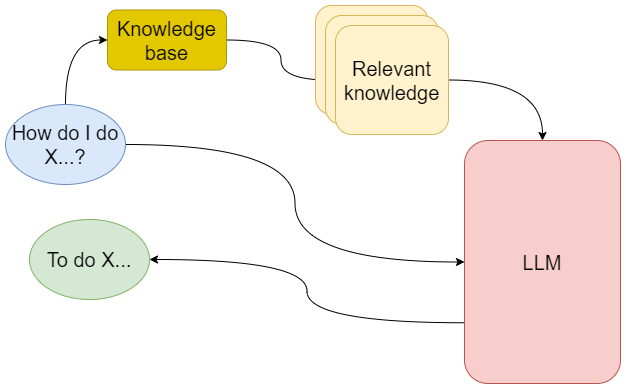
\includegraphics[width=.75\textwidth]{./Figures/RAG.png}
	\caption{Diagrama de flujo de una consulta en un chatbot con arquitectura RAG.}
	\label{fig:arquitectura_rag}
\end{figure}
% \vspace{1cm}

  \newpage
  
  \subsection{Fine-Tuning}
  El fine-tuning implica ajustar un modelo de lenguaje preentrenado en un conjunto de datos específico para mejorar su comportamiento en contextos particulares. Este proceso optimiza la efectividad del modelo en aplicaciones industriales específicas, como en medicina, derecho o ingeniería. Sin embargo, una desventaja del fine-tuning es que el modelo resultante puede quedar congelado en un estado particular, lo que limita su adaptabilidad a nuevos contextos sin un nuevo ciclo de entrenamiento.
  Aunque el fine-tuning proporciona respuestas más precisas en contextos específicos, también puede carecer de la flexibilidad de RAG, que permite incorporar datos contextuales en tiempo real.
   
  \newpage
\subsection{Ventajas y desventajas de los modelos RAG y Fine-Tuning}
  
  Esta subsección presenta una comparación entre ambos modelos, que muestra sus ventajas y desventajas.
  \begin{table}[ht]
    \centering
    \caption{Ventajas y desventajas de los modelos RAG y Fine-Tuning.}
    \begin{tabular}{|c|p{0.35\linewidth}|p{0.35\linewidth}|}
        \hline
        % \textbf{Modelo} & \textbf{Ventaja} & \textbf{Desventaja} \\
        \multicolumn{1}{|c|}{\textbf{Modelo}} & \multicolumn{1}{c|}{\textbf{Ventaja}} & \multicolumn{1}{c|}{\textbf{Desventaja}} \\ 
        \hline
        RAG & 
        \begin{raggedright}
        \begin{itemize}
            \item Permite incorporar información contextual actualizada en tiempo real.
            \item Reduce la probabilidad de alucinaciones al usar datos relevantes.
            \item Mejora la precisión y relevancia de las respuestas del chatbot.
        \end{itemize} 
        \end{raggedright} & 
        \begin{raggedright}
        \begin{itemize}
            \item Requiere una infraestructura adecuada para la recuperación de información.
            \item Dependencia de la calidad y disponibilidad de la base de datos.
            \item Puede ser más complejo de implementar y mantener.
        \end{itemize} 
        \end{raggedright} \\
        \hline
        Fine-Tuning & 
        \begin{raggedright}
        \begin{itemize}
            \item Mejora la calidad de las respuestas al adaptar el modelo a un dominio específico.
            \item Proporciona un rendimiento más consistente en contextos bien definidos.
            \item Permite la optimización de la latencia al trabajar con un modelo entrenado.
        \end{itemize} 
        \end{raggedright} & 
        \begin{raggedright}
        \begin{itemize}
            \item El modelo se congela en el tiempo y no se adapta a cambios contextuales.
            \item Requiere un conjunto de datos específico para el entrenamiento, lo que puede ser costoso.
            \item Menor flexibilidad para abordar consultas inesperadas o no entrenadas.
        \end{itemize} 
        \end{raggedright} \\
        \hline
    \end{tabular}
    \label{tab:rag_vs_finetuning}
\end{table}

  
% 	\chapter{Diseño e implementación} % Main chapter title

\label{Chapter3} % Change X to a consecutive number; for referencing this chapter elsewhere, use \ref{ChapterX}


\section{Diseño de la arquitectura} 
...
\subsection{Propuestas de implementación} 
... Descripción de los prototipos evaluados durante el diseño de la arquitectura y sus ventajas/desventajas.
\subsection{Problemas y mitigaciones} 
... Problemas con los que me he encontrado mientras realizaba cada prototipo (para dar contexto a la arquitectura elegida en el punto siguiente)
\subsection{Elección de la arquitectura de chatbot} 
... Razones por las cuales se eligió el tipo de chatbot (Fine-tuning o RAG definidos en el capitulo de Introducción Específica)


\section{Arquitectura final propuesta} 
... Descripción de la arquitectura del sistema desarrollado, incluyendo una explicación detallada de las decisiones de diseño, las distintas componentes que lo conforman, y las razones detrás de la elección de esta arquitectura. 

- - Diagrama de bloques de la arquitectura del chatbot propuesta.

\subsection{Tecnologías suplementarias} 
... Herramientas y tecnologías adicionales necesarias para el trabajo.
\subsection{Funcionamiento general} 
... Descripción completa del funcionamiento del pipeline, describiendo el camino de la pregunta desde que ingresa hasta que se genera la respuesta del chatbot.


\section{Implementación} 
\subsection{Preparación de los datos de contexto} 
... Especificación de los formatos requeridos y preprocesamiento de los datos para el entrenamiento del modelo

\subsection{Sistema de reentrenamiento con historiales} 
... Implementación del sistema para reentrenar modelos usando historiales.

- - Diagrama de flujo del sistema de reentrenamiento.


\subsection{Integración y ajustes finales del sistema} 
... Combinación de componentes y ajustes finales del sistema.


\section{Despliegue de la interfaz de pruebas} 
... Implementación de la interfaz de usuario, utilizada para realizar las pruebas en el sistema durante la etapa de desarrollo.

- - Capturas de pantalla de la interfaz de pruebas.

% \definecolor{mygreen}{rgb}{0,0.6,0}
% \definecolor{mygray}{rgb}{0.5,0.5,0.5}
% \definecolor{mymauve}{rgb}{0.58,0,0.82}

% %%%%%%%%%%%%%%%%%%%%%%%%%%%%%%%%%%%%%%%%%%%%%%%%%%%%%%%%%%%%%%%%%%%%%%%%%%%%%
% % parámetros para configurar el formato del código en los entornos lstlisting
% %%%%%%%%%%%%%%%%%%%%%%%%%%%%%%%%%%%%%%%%%%%%%%%%%%%%%%%%%%%%%%%%%%%%%%%%%%%%%
% \lstset{ %
%   backgroundcolor=\color{white},   % choose the background color; you must add \usepackage{color} or \usepackage{xcolor}
%   basicstyle=\footnotesize,        % the size of the fonts that are used for the code
%   breakatwhitespace=false,         % sets if automatic breaks should only happen at whitespace
%   breaklines=true,                 % sets automatic line breaking
%   captionpos=b,                    % sets the caption-position to bottom
%   commentstyle=\color{mygreen},    % comment style
%   deletekeywords={...},            % if you want to delete keywords from the given language
%   %escapeinside={\%*}{*)},          % if you want to add LaTeX within your code
%   %extendedchars=true,              % lets you use non-ASCII characters; for 8-bits encodings only, does not work with UTF-8
%   %frame=single,	                % adds a frame around the code
%   keepspaces=true,                 % keeps spaces in text, useful for keeping indentation of code (possibly needs columns=flexible)
%   keywordstyle=\color{blue},       % keyword style
%   language=[ANSI]C,                % the language of the code
%   %otherkeywords={*,...},           % if you want to add more keywords to the set
%   numbers=left,                    % where to put the line-numbers; possible values are (none, left, right)
%   numbersep=5pt,                   % how far the line-numbers are from the code
%   numberstyle=\tiny\color{mygray}, % the style that is used for the line-numbers
%   rulecolor=\color{black},         % if not set, the frame-color may be changed on line-breaks within not-black text (e.g. comments (green here))
%   showspaces=false,                % show spaces everywhere adding particular underscores; it overrides 'showstringspaces'
%   showstringspaces=false,          % underline spaces within strings only
%   showtabs=false,                  % show tabs within strings adding particular underscores
%   stepnumber=1,                    % the step between two line-numbers. If it's 1, each line will be numbered
%   stringstyle=\color{mymauve},     % string literal style
%   tabsize=2,	                   % sets default tabsize to 2 spaces
%   title=\lstname,                  % show the filename of files included with \lstinputlisting; also try caption instead of title
%   morecomment=[s]{/*}{*/}
% }


% %----------------------------------------------------------------------------------------
% %	SECTION 1
% %----------------------------------------------------------------------------------------
% \section{Análisis del software}
 
% La idea de esta sección es resaltar los problemas encontrados, los criterios utilizados y la justificación de las decisiones que se hayan tomado.

% Se puede agregar código o pseudocódigo dentro de un entorno lstlisting con el siguiente código:

% \begin{verbatim}
% \begin{lstlisting}[caption= "un epígrafe descriptivo"]
% 	las líneas de código irían aquí...
% \end{lstlisting}
% \end{verbatim}

% A modo de ejemplo:

% \begin{lstlisting}[label=cod:vControl,caption=Pseudocódigo del lazo principal de control.]  % Start your code-block

% #define MAX_SENSOR_NUMBER 3
% #define MAX_ALARM_NUMBER  6
% #define MAX_ACTUATOR_NUMBER 6

% uint32_t sensorValue[MAX_SENSOR_NUMBER];		
% FunctionalState alarmControl[MAX_ALARM_NUMBER];	//ENABLE or DISABLE
% state_t alarmState[MAX_ALARM_NUMBER];						//ON or OFF
% state_t actuatorState[MAX_ACTUATOR_NUMBER];			//ON or OFF

% void vControl() {

% 	initGlobalVariables();
	
% 	period = 500 ms;
		
% 	while(1) {

% 		ticks = xTaskGetTickCount();
		
% 		updateSensors();
		
% 		updateAlarms();
		
% 		controlActuators();
		
% 		vTaskDelayUntil(&ticks, period);
% 	}
% }
% \end{lstlisting}




% 	\include{Chapters/Chapter4} 
% 	\include{Chapters/Chapter5} 
% \end{verbatim}

% Los apéndices también deben escribirse en archivos .tex separados, que se deben ubicar dentro de la carpeta \emph{Appendices}. Los apéndices vienen comentados por defecto con el caracter \code{\%} y para incluirlos simplemente se debe eliminar dicho caracter.

% Finalmente, se encuentra el código para incluir la bibliografía en el documento final.  Este código tampoco debe modificarse. La metodología para trabajar las referencias bibliográficas se desarrolla en la sección \ref{sec:biblio}.
% %----------------------------------------------------------------------------------------

% \section{Bibliografía}
% \label{sec:biblio}

% Las opciones de formato de la bibliografía se controlan a través del paquete de latex \option{biblatex} que se incluye en la memoria en el archivo memoria.tex.  Estas opciones determinan cómo se generan las citas bibliográficas en el cuerpo del documento y cómo se genera la bibliografía al final de la memoria.

% En el preámbulo se puede encontrar el código que incluye el paquete biblatex, que no requiere ninguna modificación del usuario de la plantilla, y que contiene las siguientes opciones:

% \begin{lstlisting}
% \usepackage[backend=bibtex,
% 	natbib=true, 
% 	style=numeric, 
% 	sorting=none]
% {biblatex}
% \end{lstlisting}

% En el archivo \file{reference.bib} se encuentran las referencias bibliográficas que se pueden citar en el documento.  Para incorporar una nueva cita al documento lo primero es agregarla en este archivo con todos los campos necesario.  Todas las entradas bibliográficas comienzan con $@$ y una palabra que define el formato de la entrada.  Para cada formato existen campos obligatorios que deben completarse. No importa el orden en que las entradas estén definidas en el archivo .bib.  Tampoco es importante el orden en que estén definidos los campos de una entrada bibliográfica. A continuación se muestran algunos ejemplos:

% \begin{lstlisting}
% @ARTICLE{ARTICLE:1,
%     AUTHOR="John Doe",
%     TITLE="Title",
%     JOURNAL="Journal",
%     YEAR="2017",
% }
% \end{lstlisting}


% \begin{lstlisting}
% @BOOK{BOOK:1,
%     AUTHOR="John Doe",
%     TITLE="The Book without Title",
%     PUBLISHER="Dummy Publisher",
%     YEAR="2100",
% }
% \end{lstlisting}


% \begin{lstlisting}
% @INBOOK{BOOK:2,
%     AUTHOR="John Doe",
%     TITLE="The Book without Title",
%     PUBLISHER="Dummy Publisher",
%     YEAR="2100",
%     PAGES="100-200",
% }
% \end{lstlisting}


% \begin{lstlisting}
% @MISC{WEBSITE:1,
%     HOWPUBLISHED = "\url{http://example.com}",
%     AUTHOR = "Intel",
%     TITLE = "Example Website",
%     MONTH = "12",
%     YEAR = "1988",
%     URLDATE = {2012-11-26}
% }
% \end{lstlisting}

% Se debe notar que los nombres \emph{ARTICLE:1}, \emph{BOOK:1}, \emph{BOOK:2} y \emph{WEBSITE:1} son nombres de fantasía que le sirve al autor del documento para identificar la entrada. En este sentido, se podrían reemplazar por cualquier otro nombre.  Tampoco es necesario poner : seguido de un número, en los ejemplos sólo se incluye como un posible estilo para identificar las entradas.

% La entradas se citan en el documento con el comando: 

% \begin{verbatim}
% \citep{nombre_de_la_entrada}
% \end{verbatim}

% Y cuando se usan, se muestran así: \citep{ARTICLE:1}, \citep{BOOK:1}, \citep{BOOK:2}, \citep{WEBSITE:1}.  Notar cómo se conforma la sección Bibliografía al final del documento.

% Finalmente y como se mencionó en la subsección \ref{subsec:configurando}, para actualizar las referencias bibliográficas tanto en la sección bibliografía como las citas en el cuerpo del documento, se deben ejecutar las herramientas de compilación PDFLaTeX, BibTeX, PDFLaTeX, PDFLaTeX, en ese orden.  Este procedimiento debería resolver cualquier mensaje "Citation xxxxx on page x undefined".

% 	
\chapter{Introducción específica}  
 
 
Este capítulo explora los requisitos fundamentales para el desarrollo de un sistema de chatbot, que abarcan aspectos funcionales, de documentación, pruebas, interfaz y rendimiento. Además, revisa los diferentes tipos de chatbots y modelos de inteligencia artificial, con énfasis en sus características y aplicaciones en el procesamiento de lenguaje natural.


\section{Requerimientos}

\begin{enumerate}
    \item Requerimientos funcionales:
        \begin{enumerate}
            \item El sistema debe ser capaz de procesar y comprender mensajes de texto entrantes.
            \item El chatbot debe poder proporcionar respuestas relevantes y precisas a las consultas de los usuarios.
            \item Los usuarios deben tener la posibilidad de interactuar con el chatbot a través de una interfaz de usuario.
            \item Se requiere una interfaz de usuario que facilite el proceso de reentrenamiento del chatbot mediante el uso de los historiales de conversación.
        \end{enumerate}
    \item Requerimientos de documentación:
        \begin{enumerate}
            \item Documentar detalladamente las tecnologías utilizadas y sus principales características, así como las particularidades de diseño de cada una.
            \item El sistema no almacenará datos personales de los usuarios, sino que se limitará a responder preguntas frecuentes. En caso de requerirse almacenamiento de datos, se utilizará una plataforma con medidas de seguridad integradas, como autenticación mediante logins con Google.
            \item Entregar una memoria técnica que contenga información detallada sobre la implementación del sistema, que incluya aspectos técnicos, arquitectura y decisiones de diseño.
            \item Proporcionar un registro de avance que documente los hitos alcanzados durante el desarrollo del proyecto, que contemple fechas de cumplimiento y descripciones de las tareas realizadas.
         \end{enumerate}
		 
	\newpage % agrego un salto de página 
    \item Requerimientos de Testing:
        \begin{enumerate}
            \item Se llevarán a cabo pruebas en diferentes escenarios y con diferentes tipos de contexto de datos, para garantizar la fiabilidad y precisión del chatbot.
         \end{enumerate}
    \item Requerimientos de la Interfaz:
        \begin{enumerate}
            \item Se requiere una interfaz interactiva, que permita hacer preguntas y obtener respuestas en tiempo real dentro del mismo entorno de interacción.
        \end{enumerate}
    \item Requerimientos de Rendimiento:
        \begin{enumerate} 
            \item Se establece un límite máximo de tiempo de respuesta de 1 minuto, para asegurar una experiencia satisfactoria para el usuario.
        \end{enumerate}
  \end{enumerate}


  \section{Modelos de inteligencia artificial para PLN}
  El procesamiento de lenguaje natural (PLN) ha avanzado significativamente gracias al desarrollo de diversas técnicas de inteligencia artificial. Estas se pueden clasificar en varias categorías, cada una con su propio enfoque y aplicación.
     
  \textbf{Modelos basados en reglas:} estos modelos utilizan gramáticas y diccionarios para analizar el lenguaje. Aunque son efectivos en tareas específicas, su rigidez y la necesidad de una extensa programación manual limitan su aplicabilidad en contextos más amplios.
  
  \textbf{Modelos estadísticos:} a medida que los datos comenzaron a acumularse, los modelos estadísticos, como los n-gramas, se convirtieron en populares. Estos modelos predicen la probabilidad de una palabra en función de las palabras anteriores. Sin embargo, su dependencia de datos limitados puede resultar en un contexto insuficiente, lo que afecta la calidad de las predicciones.
  
  \textbf{Modelos de aprendizaje profundo:} con el auge del aprendizaje profundo, arquitecturas como RNN (Redes Neuronales Recurrentes), LSTM (Memoria a Largo Plazo) y transformers han revolucionado el PLN. Estos modelos pueden captar patrones complejos en grandes volúmenes de datos, lo que les permite realizar tareas como la traducción automática y la generación de texto de manera más efectiva.
  

  \subsection{Modelos de Lenguaje modernos}

  Modelos como BERT (Bidirectional Encoder Representations from Transformers) y GPT (Generative Pre-trained Transformer) han transformado el campo del procesamiento de lenguaje natural (PLN), al ofrecer enfoques innovadores para comprender y generar texto.
  
  \begin{itemize}
	  \item \textbf{GPT}: este modelo utiliza técnicas de aprendizaje profundo para generar texto coherente y contextualmente relevante. Su capacidad para crear respuestas naturales ha revolucionado la interacción de los chatbots con los usuarios, lo que permite conversaciones más fluidas y precisas.
  
	  \item \textbf{BERT}: a diferencia de otros modelos, BERT se centra en el análisis bidireccional del texto, lo que le permite entender el contexto de manera más profunda. Esta característica mejora la identificación de intenciones y la respuesta a preguntas complejas, lo que ayuda a crear chatbots más competentes en diálogos matizados.
  \end{itemize}
  

  \section{Modelos de chatbots: RAG vs Fine-Tuning}
  
  Los chatbots se pueden clasificar según sus arquitecturas y métodos de entrenamiento. Entre las más destacadas se encuentran Retrieval Augmented Generation (RAG) y fine-tuning. Ambas arquitecturas ofrecen ventajas complementarias, lo que las convierten en opciones populares en el desarrollo de chatbots efectivos \cite{greyling2023}.



  
  \subsection{Retrieval Augmented Generation (RAG)}
  
  RAG combina la generación de lenguaje natural con la recuperación de información, enfocándose principalmente en una \textit{knowledge base}\footnote{knowledge base [base de conocimiento].}. Cuando un usuario formula una pregunta, RAG utiliza \textit{embeddings}\footnote{embeddings [representaciones vectoriales].} para identificar y recuperar las partes del \textit{relevant knowledge}\footnote{relevant knowledge [conocimiento relevante].} que son pertinentes a esa pregunta.
  Este conocimiento relevante se inyecta en el \textit{prompt}\footnote{prompt [entrada o solicitud al modelo de lenguaje].} enviado al modelo de lenguaje (LLM). El \textit{prompt} incluye tanto la pregunta como el contexto relacionado, lo que permite a la LLM generar respuestas más precisas y contextualizadas. La incorporación de datos externos en este proceso enriquece el conocimiento del modelo en tiempo real y disminuye las posibilidades de \textit{hallucinations}\footnote{hallucinations [alucinaciones].}—respuestas que, aunque parecen plausibles, son incorrectas.
  Además, RAG utiliza bases de datos vectoriales y la búsqueda semántica para recuperar información relevante, lo que mejora la precisión y relevancia de las respuestas del chatbot. Este enfoque es especialmente útil en situaciones donde se requiere información actualizada o especializada, como en consultas de productos o en el soporte técnico.

%  \vspace{1cm}
 \begin{figure}[htbp] 
	\centering
	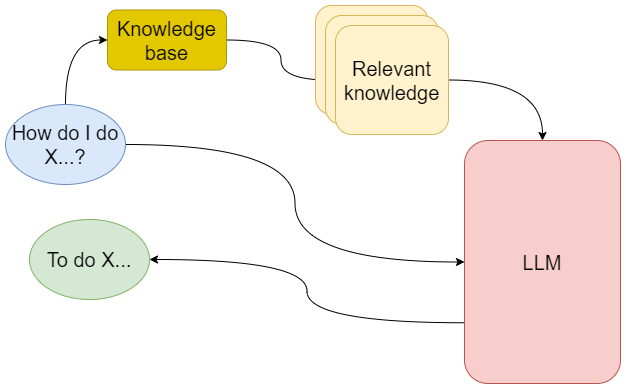
\includegraphics[width=.75\textwidth]{./Figures/RAG.png}
	\caption{Diagrama de flujo de una consulta en un chatbot con arquitectura RAG.}
	\label{fig:arquitectura_rag}
\end{figure}
% \vspace{1cm}

  \newpage
  
  \subsection{Fine-Tuning}
  El fine-tuning implica ajustar un modelo de lenguaje preentrenado en un conjunto de datos específico para mejorar su comportamiento en contextos particulares. Este proceso optimiza la efectividad del modelo en aplicaciones industriales específicas, como en medicina, derecho o ingeniería. Sin embargo, una desventaja del fine-tuning es que el modelo resultante puede quedar congelado en un estado particular, lo que limita su adaptabilidad a nuevos contextos sin un nuevo ciclo de entrenamiento.
  Aunque el fine-tuning proporciona respuestas más precisas en contextos específicos, también puede carecer de la flexibilidad de RAG, que permite incorporar datos contextuales en tiempo real.
   
  \newpage
\subsection{Ventajas y desventajas de los modelos RAG y Fine-Tuning}
  
  Esta subsección presenta una comparación entre ambos modelos, que muestra sus ventajas y desventajas.
  \begin{table}[ht]
    \centering
    \caption{Ventajas y desventajas de los modelos RAG y Fine-Tuning.}
    \begin{tabular}{|c|p{0.35\linewidth}|p{0.35\linewidth}|}
        \hline
        % \textbf{Modelo} & \textbf{Ventaja} & \textbf{Desventaja} \\
        \multicolumn{1}{|c|}{\textbf{Modelo}} & \multicolumn{1}{c|}{\textbf{Ventaja}} & \multicolumn{1}{c|}{\textbf{Desventaja}} \\ 
        \hline
        RAG & 
        \begin{raggedright}
        \begin{itemize}
            \item Permite incorporar información contextual actualizada en tiempo real.
            \item Reduce la probabilidad de alucinaciones al usar datos relevantes.
            \item Mejora la precisión y relevancia de las respuestas del chatbot.
        \end{itemize} 
        \end{raggedright} & 
        \begin{raggedright}
        \begin{itemize}
            \item Requiere una infraestructura adecuada para la recuperación de información.
            \item Dependencia de la calidad y disponibilidad de la base de datos.
            \item Puede ser más complejo de implementar y mantener.
        \end{itemize} 
        \end{raggedright} \\
        \hline
        Fine-Tuning & 
        \begin{raggedright}
        \begin{itemize}
            \item Mejora la calidad de las respuestas al adaptar el modelo a un dominio específico.
            \item Proporciona un rendimiento más consistente en contextos bien definidos.
            \item Permite la optimización de la latencia al trabajar con un modelo entrenado.
        \end{itemize} 
        \end{raggedright} & 
        \begin{raggedright}
        \begin{itemize}
            \item El modelo se congela en el tiempo y no se adapta a cambios contextuales.
            \item Requiere un conjunto de datos específico para el entrenamiento, lo que puede ser costoso.
            \item Menor flexibilidad para abordar consultas inesperadas o no entrenadas.
        \end{itemize} 
        \end{raggedright} \\
        \hline
    \end{tabular}
    \label{tab:rag_vs_finetuning}
\end{table}

  
% 	\chapter{Diseño e implementación} % Main chapter title

\label{Chapter3} % Change X to a consecutive number; for referencing this chapter elsewhere, use \ref{ChapterX}


\section{Diseño de la arquitectura} 
...
\subsection{Propuestas de implementación} 
... Descripción de los prototipos evaluados durante el diseño de la arquitectura y sus ventajas/desventajas.
\subsection{Problemas y mitigaciones} 
... Problemas con los que me he encontrado mientras realizaba cada prototipo (para dar contexto a la arquitectura elegida en el punto siguiente)
\subsection{Elección de la arquitectura de chatbot} 
... Razones por las cuales se eligió el tipo de chatbot (Fine-tuning o RAG definidos en el capitulo de Introducción Específica)


\section{Arquitectura final propuesta} 
... Descripción de la arquitectura del sistema desarrollado, incluyendo una explicación detallada de las decisiones de diseño, las distintas componentes que lo conforman, y las razones detrás de la elección de esta arquitectura. 

- - Diagrama de bloques de la arquitectura del chatbot propuesta.

\subsection{Tecnologías suplementarias} 
... Herramientas y tecnologías adicionales necesarias para el trabajo.
\subsection{Funcionamiento general} 
... Descripción completa del funcionamiento del pipeline, describiendo el camino de la pregunta desde que ingresa hasta que se genera la respuesta del chatbot.


\section{Implementación} 
\subsection{Preparación de los datos de contexto} 
... Especificación de los formatos requeridos y preprocesamiento de los datos para el entrenamiento del modelo

\subsection{Sistema de reentrenamiento con historiales} 
... Implementación del sistema para reentrenar modelos usando historiales.

- - Diagrama de flujo del sistema de reentrenamiento.


\subsection{Integración y ajustes finales del sistema} 
... Combinación de componentes y ajustes finales del sistema.


\section{Despliegue de la interfaz de pruebas} 
... Implementación de la interfaz de usuario, utilizada para realizar las pruebas en el sistema durante la etapa de desarrollo.

- - Capturas de pantalla de la interfaz de pruebas.

% \definecolor{mygreen}{rgb}{0,0.6,0}
% \definecolor{mygray}{rgb}{0.5,0.5,0.5}
% \definecolor{mymauve}{rgb}{0.58,0,0.82}

% %%%%%%%%%%%%%%%%%%%%%%%%%%%%%%%%%%%%%%%%%%%%%%%%%%%%%%%%%%%%%%%%%%%%%%%%%%%%%
% % parámetros para configurar el formato del código en los entornos lstlisting
% %%%%%%%%%%%%%%%%%%%%%%%%%%%%%%%%%%%%%%%%%%%%%%%%%%%%%%%%%%%%%%%%%%%%%%%%%%%%%
% \lstset{ %
%   backgroundcolor=\color{white},   % choose the background color; you must add \usepackage{color} or \usepackage{xcolor}
%   basicstyle=\footnotesize,        % the size of the fonts that are used for the code
%   breakatwhitespace=false,         % sets if automatic breaks should only happen at whitespace
%   breaklines=true,                 % sets automatic line breaking
%   captionpos=b,                    % sets the caption-position to bottom
%   commentstyle=\color{mygreen},    % comment style
%   deletekeywords={...},            % if you want to delete keywords from the given language
%   %escapeinside={\%*}{*)},          % if you want to add LaTeX within your code
%   %extendedchars=true,              % lets you use non-ASCII characters; for 8-bits encodings only, does not work with UTF-8
%   %frame=single,	                % adds a frame around the code
%   keepspaces=true,                 % keeps spaces in text, useful for keeping indentation of code (possibly needs columns=flexible)
%   keywordstyle=\color{blue},       % keyword style
%   language=[ANSI]C,                % the language of the code
%   %otherkeywords={*,...},           % if you want to add more keywords to the set
%   numbers=left,                    % where to put the line-numbers; possible values are (none, left, right)
%   numbersep=5pt,                   % how far the line-numbers are from the code
%   numberstyle=\tiny\color{mygray}, % the style that is used for the line-numbers
%   rulecolor=\color{black},         % if not set, the frame-color may be changed on line-breaks within not-black text (e.g. comments (green here))
%   showspaces=false,                % show spaces everywhere adding particular underscores; it overrides 'showstringspaces'
%   showstringspaces=false,          % underline spaces within strings only
%   showtabs=false,                  % show tabs within strings adding particular underscores
%   stepnumber=1,                    % the step between two line-numbers. If it's 1, each line will be numbered
%   stringstyle=\color{mymauve},     % string literal style
%   tabsize=2,	                   % sets default tabsize to 2 spaces
%   title=\lstname,                  % show the filename of files included with \lstinputlisting; also try caption instead of title
%   morecomment=[s]{/*}{*/}
% }


% %----------------------------------------------------------------------------------------
% %	SECTION 1
% %----------------------------------------------------------------------------------------
% \section{Análisis del software}
 
% La idea de esta sección es resaltar los problemas encontrados, los criterios utilizados y la justificación de las decisiones que se hayan tomado.

% Se puede agregar código o pseudocódigo dentro de un entorno lstlisting con el siguiente código:

% \begin{verbatim}
% \begin{lstlisting}[caption= "un epígrafe descriptivo"]
% 	las líneas de código irían aquí...
% \end{lstlisting}
% \end{verbatim}

% A modo de ejemplo:

% \begin{lstlisting}[label=cod:vControl,caption=Pseudocódigo del lazo principal de control.]  % Start your code-block

% #define MAX_SENSOR_NUMBER 3
% #define MAX_ALARM_NUMBER  6
% #define MAX_ACTUATOR_NUMBER 6

% uint32_t sensorValue[MAX_SENSOR_NUMBER];		
% FunctionalState alarmControl[MAX_ALARM_NUMBER];	//ENABLE or DISABLE
% state_t alarmState[MAX_ALARM_NUMBER];						//ON or OFF
% state_t actuatorState[MAX_ACTUATOR_NUMBER];			//ON or OFF

% void vControl() {

% 	initGlobalVariables();
	
% 	period = 500 ms;
		
% 	while(1) {

% 		ticks = xTaskGetTickCount();
		
% 		updateSensors();
		
% 		updateAlarms();
		
% 		controlActuators();
		
% 		vTaskDelayUntil(&ticks, period);
% 	}
% }
% \end{lstlisting}




% 	\include{Chapters/Chapter4} 
% 	\include{Chapters/Chapter5} 
% \end{verbatim}

% Los apéndices también deben escribirse en archivos .tex separados, que se deben ubicar dentro de la carpeta \emph{Appendices}. Los apéndices vienen comentados por defecto con el caracter \code{\%} y para incluirlos simplemente se debe eliminar dicho caracter.

% Finalmente, se encuentra el código para incluir la bibliografía en el documento final.  Este código tampoco debe modificarse. La metodología para trabajar las referencias bibliográficas se desarrolla en la sección \ref{sec:biblio}.
% %----------------------------------------------------------------------------------------

% \section{Bibliografía}
% \label{sec:biblio}

% Las opciones de formato de la bibliografía se controlan a través del paquete de latex \option{biblatex} que se incluye en la memoria en el archivo memoria.tex.  Estas opciones determinan cómo se generan las citas bibliográficas en el cuerpo del documento y cómo se genera la bibliografía al final de la memoria.

% En el preámbulo se puede encontrar el código que incluye el paquete biblatex, que no requiere ninguna modificación del usuario de la plantilla, y que contiene las siguientes opciones:

% \begin{lstlisting}
% \usepackage[backend=bibtex,
% 	natbib=true, 
% 	style=numeric, 
% 	sorting=none]
% {biblatex}
% \end{lstlisting}

% En el archivo \file{reference.bib} se encuentran las referencias bibliográficas que se pueden citar en el documento.  Para incorporar una nueva cita al documento lo primero es agregarla en este archivo con todos los campos necesario.  Todas las entradas bibliográficas comienzan con $@$ y una palabra que define el formato de la entrada.  Para cada formato existen campos obligatorios que deben completarse. No importa el orden en que las entradas estén definidas en el archivo .bib.  Tampoco es importante el orden en que estén definidos los campos de una entrada bibliográfica. A continuación se muestran algunos ejemplos:

% \begin{lstlisting}
% @ARTICLE{ARTICLE:1,
%     AUTHOR="John Doe",
%     TITLE="Title",
%     JOURNAL="Journal",
%     YEAR="2017",
% }
% \end{lstlisting}


% \begin{lstlisting}
% @BOOK{BOOK:1,
%     AUTHOR="John Doe",
%     TITLE="The Book without Title",
%     PUBLISHER="Dummy Publisher",
%     YEAR="2100",
% }
% \end{lstlisting}


% \begin{lstlisting}
% @INBOOK{BOOK:2,
%     AUTHOR="John Doe",
%     TITLE="The Book without Title",
%     PUBLISHER="Dummy Publisher",
%     YEAR="2100",
%     PAGES="100-200",
% }
% \end{lstlisting}


% \begin{lstlisting}
% @MISC{WEBSITE:1,
%     HOWPUBLISHED = "\url{http://example.com}",
%     AUTHOR = "Intel",
%     TITLE = "Example Website",
%     MONTH = "12",
%     YEAR = "1988",
%     URLDATE = {2012-11-26}
% }
% \end{lstlisting}

% Se debe notar que los nombres \emph{ARTICLE:1}, \emph{BOOK:1}, \emph{BOOK:2} y \emph{WEBSITE:1} son nombres de fantasía que le sirve al autor del documento para identificar la entrada. En este sentido, se podrían reemplazar por cualquier otro nombre.  Tampoco es necesario poner : seguido de un número, en los ejemplos sólo se incluye como un posible estilo para identificar las entradas.

% La entradas se citan en el documento con el comando: 

% \begin{verbatim}
% \citep{nombre_de_la_entrada}
% \end{verbatim}

% Y cuando se usan, se muestran así: \citep{ARTICLE:1}, \citep{BOOK:1}, \citep{BOOK:2}, \citep{WEBSITE:1}.  Notar cómo se conforma la sección Bibliografía al final del documento.

% Finalmente y como se mencionó en la subsección \ref{subsec:configurando}, para actualizar las referencias bibliográficas tanto en la sección bibliografía como las citas en el cuerpo del documento, se deben ejecutar las herramientas de compilación PDFLaTeX, BibTeX, PDFLaTeX, PDFLaTeX, en ese orden.  Este procedimiento debería resolver cualquier mensaje "Citation xxxxx on page x undefined".

% 
\chapter{Introducción específica}  
 
 
Este capítulo explora los requisitos fundamentales para el desarrollo de un sistema de chatbot, que abarcan aspectos funcionales, de documentación, pruebas, interfaz y rendimiento. Además, revisa los diferentes tipos de chatbots y modelos de inteligencia artificial, con énfasis en sus características y aplicaciones en el procesamiento de lenguaje natural.


\section{Requerimientos}

\begin{enumerate}
    \item Requerimientos funcionales:
        \begin{enumerate}
            \item El sistema debe ser capaz de procesar y comprender mensajes de texto entrantes.
            \item El chatbot debe poder proporcionar respuestas relevantes y precisas a las consultas de los usuarios.
            \item Los usuarios deben tener la posibilidad de interactuar con el chatbot a través de una interfaz de usuario.
            \item Se requiere una interfaz de usuario que facilite el proceso de reentrenamiento del chatbot mediante el uso de los historiales de conversación.
        \end{enumerate}
    \item Requerimientos de documentación:
        \begin{enumerate}
            \item Documentar detalladamente las tecnologías utilizadas y sus principales características, así como las particularidades de diseño de cada una.
            \item El sistema no almacenará datos personales de los usuarios, sino que se limitará a responder preguntas frecuentes. En caso de requerirse almacenamiento de datos, se utilizará una plataforma con medidas de seguridad integradas, como autenticación mediante logins con Google.
            \item Entregar una memoria técnica que contenga información detallada sobre la implementación del sistema, que incluya aspectos técnicos, arquitectura y decisiones de diseño.
            \item Proporcionar un registro de avance que documente los hitos alcanzados durante el desarrollo del proyecto, que contemple fechas de cumplimiento y descripciones de las tareas realizadas.
         \end{enumerate}
		 
	\newpage % agrego un salto de página 
    \item Requerimientos de Testing:
        \begin{enumerate}
            \item Se llevarán a cabo pruebas en diferentes escenarios y con diferentes tipos de contexto de datos, para garantizar la fiabilidad y precisión del chatbot.
         \end{enumerate}
    \item Requerimientos de la Interfaz:
        \begin{enumerate}
            \item Se requiere una interfaz interactiva, que permita hacer preguntas y obtener respuestas en tiempo real dentro del mismo entorno de interacción.
        \end{enumerate}
    \item Requerimientos de Rendimiento:
        \begin{enumerate} 
            \item Se establece un límite máximo de tiempo de respuesta de 1 minuto, para asegurar una experiencia satisfactoria para el usuario.
        \end{enumerate}
  \end{enumerate}


  \section{Modelos de inteligencia artificial para PLN}
  El procesamiento de lenguaje natural (PLN) ha avanzado significativamente gracias al desarrollo de diversas técnicas de inteligencia artificial. Estas se pueden clasificar en varias categorías, cada una con su propio enfoque y aplicación.
     
  \textbf{Modelos basados en reglas:} estos modelos utilizan gramáticas y diccionarios para analizar el lenguaje. Aunque son efectivos en tareas específicas, su rigidez y la necesidad de una extensa programación manual limitan su aplicabilidad en contextos más amplios.
  
  \textbf{Modelos estadísticos:} a medida que los datos comenzaron a acumularse, los modelos estadísticos, como los n-gramas, se convirtieron en populares. Estos modelos predicen la probabilidad de una palabra en función de las palabras anteriores. Sin embargo, su dependencia de datos limitados puede resultar en un contexto insuficiente, lo que afecta la calidad de las predicciones.
  
  \textbf{Modelos de aprendizaje profundo:} con el auge del aprendizaje profundo, arquitecturas como RNN (Redes Neuronales Recurrentes), LSTM (Memoria a Largo Plazo) y transformers han revolucionado el PLN. Estos modelos pueden captar patrones complejos en grandes volúmenes de datos, lo que les permite realizar tareas como la traducción automática y la generación de texto de manera más efectiva.
  

  \subsection{Modelos de Lenguaje modernos}

  Modelos como BERT (Bidirectional Encoder Representations from Transformers) y GPT (Generative Pre-trained Transformer) han transformado el campo del procesamiento de lenguaje natural (PLN), al ofrecer enfoques innovadores para comprender y generar texto.
  
  \begin{itemize}
	  \item \textbf{GPT}: este modelo utiliza técnicas de aprendizaje profundo para generar texto coherente y contextualmente relevante. Su capacidad para crear respuestas naturales ha revolucionado la interacción de los chatbots con los usuarios, lo que permite conversaciones más fluidas y precisas.
  
	  \item \textbf{BERT}: a diferencia de otros modelos, BERT se centra en el análisis bidireccional del texto, lo que le permite entender el contexto de manera más profunda. Esta característica mejora la identificación de intenciones y la respuesta a preguntas complejas, lo que ayuda a crear chatbots más competentes en diálogos matizados.
  \end{itemize}
  

  \section{Modelos de chatbots: RAG vs Fine-Tuning}
  
  Los chatbots se pueden clasificar según sus arquitecturas y métodos de entrenamiento. Entre las más destacadas se encuentran Retrieval Augmented Generation (RAG) y fine-tuning. Ambas arquitecturas ofrecen ventajas complementarias, lo que las convierten en opciones populares en el desarrollo de chatbots efectivos \cite{greyling2023}.



  
  \subsection{Retrieval Augmented Generation (RAG)}
  
  RAG combina la generación de lenguaje natural con la recuperación de información, enfocándose principalmente en una \textit{knowledge base}\footnote{knowledge base [base de conocimiento].}. Cuando un usuario formula una pregunta, RAG utiliza \textit{embeddings}\footnote{embeddings [representaciones vectoriales].} para identificar y recuperar las partes del \textit{relevant knowledge}\footnote{relevant knowledge [conocimiento relevante].} que son pertinentes a esa pregunta.
  Este conocimiento relevante se inyecta en el \textit{prompt}\footnote{prompt [entrada o solicitud al modelo de lenguaje].} enviado al modelo de lenguaje (LLM). El \textit{prompt} incluye tanto la pregunta como el contexto relacionado, lo que permite a la LLM generar respuestas más precisas y contextualizadas. La incorporación de datos externos en este proceso enriquece el conocimiento del modelo en tiempo real y disminuye las posibilidades de \textit{hallucinations}\footnote{hallucinations [alucinaciones].}—respuestas que, aunque parecen plausibles, son incorrectas.
  Además, RAG utiliza bases de datos vectoriales y la búsqueda semántica para recuperar información relevante, lo que mejora la precisión y relevancia de las respuestas del chatbot. Este enfoque es especialmente útil en situaciones donde se requiere información actualizada o especializada, como en consultas de productos o en el soporte técnico.

%  \vspace{1cm}
 \begin{figure}[htbp] 
	\centering
	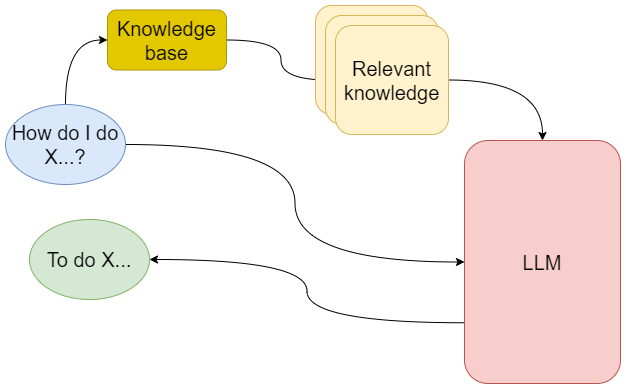
\includegraphics[width=.75\textwidth]{./Figures/RAG.png}
	\caption{Diagrama de flujo de una consulta en un chatbot con arquitectura RAG.}
	\label{fig:arquitectura_rag}
\end{figure}
% \vspace{1cm}

  \newpage
  
  \subsection{Fine-Tuning}
  El fine-tuning implica ajustar un modelo de lenguaje preentrenado en un conjunto de datos específico para mejorar su comportamiento en contextos particulares. Este proceso optimiza la efectividad del modelo en aplicaciones industriales específicas, como en medicina, derecho o ingeniería. Sin embargo, una desventaja del fine-tuning es que el modelo resultante puede quedar congelado en un estado particular, lo que limita su adaptabilidad a nuevos contextos sin un nuevo ciclo de entrenamiento.
  Aunque el fine-tuning proporciona respuestas más precisas en contextos específicos, también puede carecer de la flexibilidad de RAG, que permite incorporar datos contextuales en tiempo real.
   
  \newpage
\subsection{Ventajas y desventajas de los modelos RAG y Fine-Tuning}
  
  Esta subsección presenta una comparación entre ambos modelos, que muestra sus ventajas y desventajas.
  \begin{table}[ht]
    \centering
    \caption{Ventajas y desventajas de los modelos RAG y Fine-Tuning.}
    \begin{tabular}{|c|p{0.35\linewidth}|p{0.35\linewidth}|}
        \hline
        % \textbf{Modelo} & \textbf{Ventaja} & \textbf{Desventaja} \\
        \multicolumn{1}{|c|}{\textbf{Modelo}} & \multicolumn{1}{c|}{\textbf{Ventaja}} & \multicolumn{1}{c|}{\textbf{Desventaja}} \\ 
        \hline
        RAG & 
        \begin{raggedright}
        \begin{itemize}
            \item Permite incorporar información contextual actualizada en tiempo real.
            \item Reduce la probabilidad de alucinaciones al usar datos relevantes.
            \item Mejora la precisión y relevancia de las respuestas del chatbot.
        \end{itemize} 
        \end{raggedright} & 
        \begin{raggedright}
        \begin{itemize}
            \item Requiere una infraestructura adecuada para la recuperación de información.
            \item Dependencia de la calidad y disponibilidad de la base de datos.
            \item Puede ser más complejo de implementar y mantener.
        \end{itemize} 
        \end{raggedright} \\
        \hline
        Fine-Tuning & 
        \begin{raggedright}
        \begin{itemize}
            \item Mejora la calidad de las respuestas al adaptar el modelo a un dominio específico.
            \item Proporciona un rendimiento más consistente en contextos bien definidos.
            \item Permite la optimización de la latencia al trabajar con un modelo entrenado.
        \end{itemize} 
        \end{raggedright} & 
        \begin{raggedright}
        \begin{itemize}
            \item El modelo se congela en el tiempo y no se adapta a cambios contextuales.
            \item Requiere un conjunto de datos específico para el entrenamiento, lo que puede ser costoso.
            \item Menor flexibilidad para abordar consultas inesperadas o no entrenadas.
        \end{itemize} 
        \end{raggedright} \\
        \hline
    \end{tabular}
    \label{tab:rag_vs_finetuning}
\end{table}

  
% \chapter{Diseño e implementación} % Main chapter title

\label{Chapter3} % Change X to a consecutive number; for referencing this chapter elsewhere, use \ref{ChapterX}


\section{Diseño de la arquitectura} 
...
\subsection{Propuestas de implementación} 
... Descripción de los prototipos evaluados durante el diseño de la arquitectura y sus ventajas/desventajas.
\subsection{Problemas y mitigaciones} 
... Problemas con los que me he encontrado mientras realizaba cada prototipo (para dar contexto a la arquitectura elegida en el punto siguiente)
\subsection{Elección de la arquitectura de chatbot} 
... Razones por las cuales se eligió el tipo de chatbot (Fine-tuning o RAG definidos en el capitulo de Introducción Específica)


\section{Arquitectura final propuesta} 
... Descripción de la arquitectura del sistema desarrollado, incluyendo una explicación detallada de las decisiones de diseño, las distintas componentes que lo conforman, y las razones detrás de la elección de esta arquitectura. 

- - Diagrama de bloques de la arquitectura del chatbot propuesta.

\subsection{Tecnologías suplementarias} 
... Herramientas y tecnologías adicionales necesarias para el trabajo.
\subsection{Funcionamiento general} 
... Descripción completa del funcionamiento del pipeline, describiendo el camino de la pregunta desde que ingresa hasta que se genera la respuesta del chatbot.


\section{Implementación} 
\subsection{Preparación de los datos de contexto} 
... Especificación de los formatos requeridos y preprocesamiento de los datos para el entrenamiento del modelo

\subsection{Sistema de reentrenamiento con historiales} 
... Implementación del sistema para reentrenar modelos usando historiales.

- - Diagrama de flujo del sistema de reentrenamiento.


\subsection{Integración y ajustes finales del sistema} 
... Combinación de componentes y ajustes finales del sistema.


\section{Despliegue de la interfaz de pruebas} 
... Implementación de la interfaz de usuario, utilizada para realizar las pruebas en el sistema durante la etapa de desarrollo.

- - Capturas de pantalla de la interfaz de pruebas.

% \definecolor{mygreen}{rgb}{0,0.6,0}
% \definecolor{mygray}{rgb}{0.5,0.5,0.5}
% \definecolor{mymauve}{rgb}{0.58,0,0.82}

% %%%%%%%%%%%%%%%%%%%%%%%%%%%%%%%%%%%%%%%%%%%%%%%%%%%%%%%%%%%%%%%%%%%%%%%%%%%%%
% % parámetros para configurar el formato del código en los entornos lstlisting
% %%%%%%%%%%%%%%%%%%%%%%%%%%%%%%%%%%%%%%%%%%%%%%%%%%%%%%%%%%%%%%%%%%%%%%%%%%%%%
% \lstset{ %
%   backgroundcolor=\color{white},   % choose the background color; you must add \usepackage{color} or \usepackage{xcolor}
%   basicstyle=\footnotesize,        % the size of the fonts that are used for the code
%   breakatwhitespace=false,         % sets if automatic breaks should only happen at whitespace
%   breaklines=true,                 % sets automatic line breaking
%   captionpos=b,                    % sets the caption-position to bottom
%   commentstyle=\color{mygreen},    % comment style
%   deletekeywords={...},            % if you want to delete keywords from the given language
%   %escapeinside={\%*}{*)},          % if you want to add LaTeX within your code
%   %extendedchars=true,              % lets you use non-ASCII characters; for 8-bits encodings only, does not work with UTF-8
%   %frame=single,	                % adds a frame around the code
%   keepspaces=true,                 % keeps spaces in text, useful for keeping indentation of code (possibly needs columns=flexible)
%   keywordstyle=\color{blue},       % keyword style
%   language=[ANSI]C,                % the language of the code
%   %otherkeywords={*,...},           % if you want to add more keywords to the set
%   numbers=left,                    % where to put the line-numbers; possible values are (none, left, right)
%   numbersep=5pt,                   % how far the line-numbers are from the code
%   numberstyle=\tiny\color{mygray}, % the style that is used for the line-numbers
%   rulecolor=\color{black},         % if not set, the frame-color may be changed on line-breaks within not-black text (e.g. comments (green here))
%   showspaces=false,                % show spaces everywhere adding particular underscores; it overrides 'showstringspaces'
%   showstringspaces=false,          % underline spaces within strings only
%   showtabs=false,                  % show tabs within strings adding particular underscores
%   stepnumber=1,                    % the step between two line-numbers. If it's 1, each line will be numbered
%   stringstyle=\color{mymauve},     % string literal style
%   tabsize=2,	                   % sets default tabsize to 2 spaces
%   title=\lstname,                  % show the filename of files included with \lstinputlisting; also try caption instead of title
%   morecomment=[s]{/*}{*/}
% }


% %----------------------------------------------------------------------------------------
% %	SECTION 1
% %----------------------------------------------------------------------------------------
% \section{Análisis del software}
 
% La idea de esta sección es resaltar los problemas encontrados, los criterios utilizados y la justificación de las decisiones que se hayan tomado.

% Se puede agregar código o pseudocódigo dentro de un entorno lstlisting con el siguiente código:

% \begin{verbatim}
% \begin{lstlisting}[caption= "un epígrafe descriptivo"]
% 	las líneas de código irían aquí...
% \end{lstlisting}
% \end{verbatim}

% A modo de ejemplo:

% \begin{lstlisting}[label=cod:vControl,caption=Pseudocódigo del lazo principal de control.]  % Start your code-block

% #define MAX_SENSOR_NUMBER 3
% #define MAX_ALARM_NUMBER  6
% #define MAX_ACTUATOR_NUMBER 6

% uint32_t sensorValue[MAX_SENSOR_NUMBER];		
% FunctionalState alarmControl[MAX_ALARM_NUMBER];	//ENABLE or DISABLE
% state_t alarmState[MAX_ALARM_NUMBER];						//ON or OFF
% state_t actuatorState[MAX_ACTUATOR_NUMBER];			//ON or OFF

% void vControl() {

% 	initGlobalVariables();
	
% 	period = 500 ms;
		
% 	while(1) {

% 		ticks = xTaskGetTickCount();
		
% 		updateSensors();
		
% 		updateAlarms();
		
% 		controlActuators();
		
% 		vTaskDelayUntil(&ticks, period);
% 	}
% }
% \end{lstlisting}




% \include{Chapters/Chapter4} 
% \include{Chapters/Chapter5} 

% ----------------------------------------------------------------------------------------
% 	CONTENIDO DE LA MEMORIA  - APÉNDICES
% ----------------------------------------------------------------------------------------

% \appendix % indicativo para indicarle a LaTeX los siguientes "capítulos" son apéndices

% Incluir los apéndices de la memoria como archivos separadas desde la carpeta Appendices
% Descomentar las líneas a medida que se escriben los apéndices

% \include{Appendices/AppendixA}
% \include{Appendices/AppendixB}
% \include{Appendices/AppendixC}

%----------------------------------------------------------------------------------------
%	BIBLIOGRAPHY
%----------------------------------------------------------------------------------------

\Urlmuskip=0mu plus 1mu\relax
\raggedright
\printbibliography[heading=bibintoc]

%----------------------------------------------------------------------------------------

\end{document}  
